\documentclass{article}
\usepackage{amsmath,amssymb,amsthm}
\usepackage{color}
\usepackage{hyperref}
\usepackage{stmaryrd}
\usepackage{float}
\usepackage{listings}
\usepackage{graphicx}
\usepackage{fullpage}
\usepackage{times}
\usepackage{lscape}
\usepackage{setspace}

% Stuff needed for typesetting lambdaLVish and its metatheory
%%% Macros for typesetting terms of the LVish language itself.

% Sans-serif font for terms of the language
\newcommand\termfont[1]{\mbox{\texttt{#1}}}

% Amount to indent the next line of a 'let' expression.
\newcommand{\letspace}{\hspace{1.1em}}
\newcommand{\letparspace}{\hspace{3.7em}}

%%% Language forms.

\newcommand{\lam}[2]{\ensuremath{\lambda#1.\,#2}}
\newcommand{\app}[2]{\ensuremath{#1~#2}}

\newcommand{\unit}{\termfont{()}}

\newcommand{\NEW}{\termfont{new}}

\newcommand{\PUT}{\termfont{put}}
\newcommand{\putexp}[2]{\ensuremath{\PUT~#1~#2}}

\newcommand{\GET}{\termfont{get}}
\newcommand{\getexp}[2]{\ensuremath{\GET~#1~#2}}

\newcommand{\BUMP}{\termfont{bump}}
\newcommand{\bumpexp}[1]{\ensuremath{\BUMP~#1}}

\newcommand{\GETFSTORSND}{\termfont{getFstOrSnd}}
\newcommand{\GETFST}{\termfont{getFst}}
\newcommand{\getfstexp}[1]{\ensuremath{\GETFST~#1}}
\newcommand{\GETSND}{\termfont{getSnd}}
\newcommand{\getsndexp}[1]{\ensuremath{\GETSND~#1}}

\newcommand{\FREEZE}{\termfont{freeze}}
\newcommand{\AFTER}{~{\termfont{after}}}
\newcommand{\WITH}{~{\termfont{with}}}

\newcommand{\ADDHANDLER}{{\termfont{addHandler}}}
\newcommand{\NEWPOOL}{{\termfont{newPool}}}
\newcommand{\ADDHANDLERINPOOL}{{\termfont{addInPool}}}
\newcommand{\QUIESCE}{{\termfont{quiesce}}}

\newcommand{\FAW}{{\termfont{freeze}-\termfont{after}-\termfont{with}}}
\newcommand{\freeze}[1]{\ensuremath{\FREEZE~#1}}
\newcommand{\freezeafter}[3]{\ensuremath{\FREEZE~#1~\AFTER~#2~\WITH~#3}}
\newcommand{\freezeafterfull}[5]{\ensuremath{\FREEZE~#1~\AFTER~#2~\WITH~#3, #4, #5}}

\newcommand{\LET}{\termfont{let}}
\newcommand{\PAR}{\termfont{par}}
\newcommand{\LETPAR}{\termfont{\LET~\PAR}}
\newcommand{\IN}{\termfont{in}}
\newcommand{\letexp}[3]{\ensuremath{\LET~#1=#2~\IN~#3}}
\newcommand{\letparexp}[5]{\ensuremath{\LETPAR~#1=#2;~#3=#4~\IN~#5}}

\newcommand{\stateset}[1]{\ensuremath{\lbrace #1 \rbrace}}

\newcommand{\UNIQUE}{\termfont{unique}}

\newcommand{\lambdalvar}{\ensuremath{\lambda_{\textsf{LVar}}}}


%%% Macros for typesetting lambdaLVar and lambdaLVish semantics and metatheory.

%%% Names of the languages.
\newcommand{\lambdaLVar}{\ensuremath{\lambda_{\textrm{LVar}}}}
\newcommand{\lambdaLVish}{\ensuremath{\lambda_{\textrm{LVish}}}}

%%% BNF grammar stuff
\newcommand{\bnfdef}{\ensuremath{::=}}
\newcommand{\bnfsep}{\ensuremath{\ \ | \ \ }}
\newcommand{\setsep}{\ensuremath{\ | \ }}
\newcommand{\sep}{\bnfsep}

%%% Metafunctions
\newcommand{\subst}[3]{\ensuremath{#1[#2 := #3]}}
\newcommand{\dom}[1]{\ensuremath{\mathit{dom}(#1)}}
\newcommand{\incomp}[1]{\ensuremath{\mathit{incomp}(#1)}}
\newcommand{\pred}[1]{\ensuremath{\mathit{pred}(#1)}}
\newcommand{\userlub}[2]{\ensuremath{#1 \sqcup #2}}
\newcommand{\lubp}[2]{\ensuremath{#1 \sqcup_p #2}}
\newcommand{\qexist}[2]{\ensuremath{\exists\,#1.~#2}}
\newcommand{\qforall}[2]{\ensuremath{\forall\,#1.~#2}}
\newcommand{\userelements}{\ensuremath{\mathit{Elements}}}
\newcommand{\userleq}{\ensuremath{\sqsubseteq}}
\newcommand{\nuserleq}{\ensuremath{\not \sqsubseteq}}
\newcommand{\usergeq}{\ensuremath{\sqsupseteq}}
\newcommand{\userlt}{\ensuremath{\sqsubset}}
\newcommand{\leqp}{\ensuremath{\sqsubseteq_p}}
\newcommand{\ltp}{\ensuremath{\sqsubset_p}}
\newcommand{\botp}{\ensuremath{\bot_{p}}}
\newcommand{\topp}{\ensuremath{\top\hspace{-0.85mm}_{p}}}

%%% Evaluation / operational semantics
\newcommand*{\longhookrightarrow}{\ensuremath{\lhook\joinrel\relbar\joinrel\rightarrow}}

%%% Reduction semantics evaluation relation
\newcommand{\parstepsto}{\ensuremath{\longhookrightarrow}}
\newcommand{\parstepstoeq}{\ensuremath{\longhookrightarrow^{?}}}

%%% Context semantics evaluation relation
\newcommand{\ctxstepsto}{\ensuremath{\longmapsto}}

\newcommand{\evalctxt}[2]{\ensuremath{#1\hspace{-0.5mm}\left[#2\right]}}
\newcommand{\E}[1]{\ensuremath{\evalctxt{E}{#1}}}

%%% Stores and store operations
\newcommand{\storeS}{\ensuremath{\mathrm{S}}}
\newcommand{\StoreVal}{\ensuremath{\mathit{StoreVal}}}
\newcommand{\fmap}{\ensuremath{\stackrel{\textrm{fin}}{\rightarrow}}}
\newcommand{\eqstore}[2]{\ensuremath{#1 =_{\storeS} #2}}
\newcommand{\leqstore}[2]{\ensuremath{#1 \userleq_{\storeS} #2}}
\newcommand{\neqstore}[2]{\ensuremath{#1 \not =_{\storeS} #2}}
\newcommand{\nleqstore}[2]{\ensuremath{#1 \not \userleq_{\storeS} #2}}
\newcommand{\ltstore}[2]{\ensuremath{#1 \userlt_{\storeS} #2}}
\newcommand{\lubstore}[2]{\ensuremath{#1 \sqcup_{\storeS} #2}}
\newcommand{\glbstore}[2]{\ensuremath{#1 \sqcap_{\storeS} #2}}
\newcommand{\storebindingRaw}[2]{\ensuremath{#1 \mapsto #2}}
\newcommand{\storebinding}[3]{\storebindingRaw{#1}{\state{#2}{#3}}}
\newcommand{\state}[2]{\ensuremath{(#1, #2)}}
\newcommand{\store}[1]{\left[ #1 \right]}
\newcommand{\extS}[4]{#1[\storebinding{#2}{#3}{#4}]}
\newcommand{\extSRaw}[3]{#1[\storebindingRaw{#2}{#3}]}
\newcommand{\storeset}{\mathcal{S}}
\newcommand{\status}{\ensuremath{\mathit{frz}}}
\newcommand{\frozentrue}{\ensuremath{\textsf{true}}}
\newcommand{\frozenfalse}{\ensuremath{\textsf{false}}}
\newcommand{\Loc}{\mathit{Loc}}
\newcommand{\topS}{\ensuremath{\top\hspace{-0.85mm}_{\storeS}}}
\newcommand{\LVar}{\mathit{LVar}}

%% It would be really nice to be able to typeset stores like

%%        \store{l_1, l_2, l_3}{3, 4, 5}

%% producing

%%        {l_1 -> 3, l_2 -> 4, l_3 -> 5}

%% but to do that, I think we need something like what's done in
%% http://stackoverflow.com/questions/2402354/split-comma-separated-parameters-in-latex,
%% and I haven't figured out how to do it just yet :(

%%% States and configurations
\newcommand{\conf}{\ensuremath{\sigma}}
\newcommand{\config}[2]{\ensuremath{\langle #1;\, #2 \rangle}}
\newcommand{\error}{\ensuremath{\textbf{\textsf{error}}}}

\newcommand{\handledBy}{\hookrightarrow}

%%% Assorted math stuff
\newcommand{\defeq}{\stackrel{\triangle}{=}} % "defined-as"
\newcommand{\pfn}{\rightharpoonup}
\newcommand{\bag}[1]{\Lbag #1 \Rbag}
\newcommand{\setof}[1]{\left\{#1\right\}}
\newcommand{\comprehend}[2]{\setof{{#1}\;\middle|\;{#2}}}
\newcommand{\power}[1]{\mathcal{P}(#1)}
\newcommand{\inlop}{\mathsf{inl}}
\newcommand{\inl}[1]{\inlop\,{#1}}
\newcommand{\inrop}{\mathsf{inr}}
\newcommand{\inr}[1]{\inrop\,{#1}}
\newcommand{\letv}[2]{\mathsf{let}\;{#1} = {#2}}
\newcommand{\Freeze}[1]{\mathrm{Freeze}(#1)}
\newcommand{\piinv}{\pi^{-1}}
\newcommand{\piprimeinv}{\pi'^{-1}}
\newcommand{\andlv}[2]{\ensuremath{(\texttt{#1},\texttt{#2})}}
\newcommand{\id}{\mathrm{id}}
\newcommand{\eventually}{\lozenge}
\newcommand{\block}{\textsf{block}}


% For typesetting inference rules
\usepackage{../latex_common/mathpartir}

% Syntax and semantics of lambdaLVish, specific to this proposal (the
% semantics was later replaced by one split into a reduction semantics
% and a context semantics, plus some other generalizations)
\newcommand{\FigLambdaLVishGrammar}[1][t]{
\begin{figure}[#1]
  Given a lattice $(D, \userleq, \bot, \top)$ with elements $d \in D$:
{\doublespacing
    \[
    \begin{array}{rlcl}
      \mbox{configurations} & \conf & \bnfdef & \config{S}{e} \sep \error \\
      \mbox{expressions} & e & \bnfdef & 
           x \sep 
           v \sep 
           \app{e}{e} \sep 
           \getexp{e}{e} \sep 
           \putiexp{e} \sep
           \NEW \sep
           \freeze{e} \\
           & & \sep &
           \freezeafter{e}{e}{e} \\
           & & \sep &
           \freezeafterfull{l}{Q}{\lam{x}{e}}{\setof{e, \dots}}{H} \\
      \mbox{values} & v & \bnfdef & \unit \sep d \sep p \sep l \sep P \sep Q \sep \lam{x}{e} \\
      \mbox{threshold sets} & P & \bnfdef & \stateset{p_1,\,p_2,\,\dots} \\
      \mbox{event sets} & Q & \bnfdef & \stateset{d_1,\,d_2,\,\dots} \\
      \mbox{``handled'' sets} & H & \bnfdef & \setof{d_1,\,\dots, d_n} \\
      %% N.B. In Redex we actually rule out store values being Top in
      %% the grammar, and have a special StoreVal type for elements
      %% other than Top.  Here we don't bother, and we just say that
      %% stores contain bindings from locations l to pairs p.
      \mbox{stores} & S & \bnfdef &
        \store{\storebindingRaw{l_1}{p_1},\,\dots, \storebindingRaw{l_n}{p_n}} \sep \topS \\
      \mbox{states} & p & \bnfdef & \state{d}{\status} \\
      \mbox{status bits} & \status & \bnfdef & \frozentrue \sep \frozenfalse \\
      \mbox{evaluation contexts} & E & \bnfdef &
           [~] \sep
           \app{E}{e} \sep
           \app{e}{E} \sep
           \getexp{E}{e} \sep
           \getexp{e}{E} \sep 
           \putiexp{E} \\
           & & \sep &
           \freeze {E} \sep
           \freezeafter{E}{e}{e} \\
           & & \sep &
           \freezeafter{e}{E}{e} \sep
           \freezeafter{e}{e}{E} \\
           & & \sep &
           \freezeafterfull{v}{v}{v}{\setof{e\dots~E~e\dots}}{H}
    \end{array}           
    \]
}
  \caption{Syntax for $\lambdaLVish$.}
  \label{f:lambdaLVish-syntax}
\end{figure}
}

\newcommand{\FigLambdaLVishSemantics}[1][t]{
\begin{landscape}
\begin{figure}[#1]
  Given a lattice $(D, \userleq, \bot, \top)$ with elements $d \in D$: \\
{\doublespacing
  \begin{mathpar}
    \inferrule*[lab=E-Eval-Ctxt]
        {\config{S}{e} \parstepsto \config{S'}{e'}}
        {\config{S}{\E{e}} \parstepsto \config{S'}{\E{e'}}}

    \inferrule*[lab=E-Beta]
        {~}
        {\config{S}{\app{(\lam{x}{e})}{v}} \parstepsto \config{S}{\subst{e}{x}{v}}}

    \inferrule*[lab=E-New, right=\textnormal{($l \notin \dom{S}$)}]
        {~}
        {\config{S}{\NEW} \parstepsto \config{\extS{S}{l}{\bot}{\frozenfalse}}{l}}

    \inferrule*[lab=E-Put]
        {S(l) = p_1 \\ u_{p_i}(p_1) \neq \topp}
        {\config{S}{\putiexp{l}} \parstepsto
          \config{\extSRaw{S}{l}{u_{p_i}(p_1)}}{\unit}}

    \inferrule*[lab=E-Put-Err]
        {S(l) = p_1 \\ u_{p_i}(p_1) = \topp}
        {\config{S}{\putiexp{l}} \parstepsto \error}

    \inferrule*[lab=E-Get]
        {S(l) = p_1 \\ \incomp{P} \\ p_2 \in P \\ p_2 \leqp p_1}
        {\config{S}{\getexp{l}{P}} \parstepsto \config{S}{p_2}}

    \inferrule*[lab=E-Freeze-Init]
        {~}
        {\config{S}{\freezeafter{l}{Q}{\lam{x}{e}}} \parstepsto
          \config{S}{\freezeafterfull{l}{Q}{\lam{x}{e}}{\setof{}}{\setof{}}}}

    \inferrule*[lab=E-Spawn-Handler]
        { S(l) = \state{d_1}{\status_1} \\ 
          d_2 \userleq d_1 \\
          d_2 \notin H \\
          d_2 \in Q
        }
        {
          \config{S}{\freezeafterfull{l}{Q}{\lam{x}{e_0}}{\setof{e, \dots}}{H}}
          \parstepsto
          \config{S}{\freezeafterfull{l}{Q}{\lam{x}{e_0}}{\setof{\subst{e_0}{x}{d_2}, e, \dots}}
            {\{d_2\}\cup H}}
        }

    \inferrule*[lab=E-Freeze-Final]
        { S(l) = \state{d_1}{\status_1} \\ 
          \forall{d_2} ~.~ ( {d_2 \userleq d_1 \land d_2 \in Q} \Rightarrow 
             d_2 \in H) }
        {
          \config{S}{\freezeafterfull{l}{Q}{v}{\setof{v\dots}}{H}}
          \parstepsto
          \config{\extS{S}{l}{d_1}{\frozentrue}}{d_1}
        }

    \inferrule*[lab=E-Freeze-Simple]
        { S(l) = \state{d_1}{\status_1} }
        {
          \config{S}{\freeze{l}}
          \parstepsto
          \config{\extS{S}{l}{d_1}{\frozentrue}}{d_1}
        }
  \end{mathpar}
}
  \caption{Reduction semantics for $\lambdaLVish$.}
  \label{f:lambdaLVish-semantics}
\end{figure}
\end{landscape}
}

% Language stuff that's specific to this proposal
\newcommand{\bumpexp}[1]{\ensuremath{\termfont{bump}~#1}}

% Definitions, lemmas, theorems
\newcommand{\DefStability}{
  \begin{definition}[Stable Configurations]
    A configuration $\config{S}{e}$ is \emph{stable} if the free locations of $e$ are a subset of $\dom{S}$. 
  \end{definition}
}

\newcommand{\DefLatticeWithStatusBits}{
\begin{definition}\label{def:lattice-with-status-bits}
Suppose $(D, \userleq, \bot, \top)$ is a lattice.  We define an
operation $\Freeze{D, \userleq, \bot, \top} \defeq (D_p, \leqp, \botp,
\topp)$ as follows:
\begin{enumerate}
\item $D_p$ is a set defined as follows:
\begin{equation*}
\begin{split}
  D_p  \defeq & \setof{ \state{d}{\status} \sep d \in (D - \setof{\top}) \land \status
    \in \setof{\frozentrue, \frozenfalse} } \\
  & \cup \setof{(\top, \frozenfalse)}
\end{split}
\end{equation*}

\item $\leqp \;\in\, \power{D_p \times D_p}$ is a binary relation
  defined as follows:
\begin{displaymath}
  \begin{array}{lclcl}
    \state{d}{\frozenfalse} & \leqp & \state{d'}{\frozenfalse} & \iff & d \userleq d' \\ 
    \state{d}{\frozentrue} & \leqp & \state{d'}{\frozentrue} & \iff & d = d' \\
    \state{d}{\frozenfalse} & \leqp & \state{d'}{\frozentrue}  & \iff & d \userleq d' \\
    \state{d}{\frozentrue} & \leqp & \state{d'}{\frozenfalse}  & \iff & d' = \top 
  \end{array}
\end{displaymath}

\item $\botp \defeq \state{\bot}{\frozenfalse}$.

\item $\topp \defeq \state{\top}{\frozenfalse}$.
\end{enumerate}
\end{definition}
}

\newcommand{\DefLubP}{
\begin{definition}\label{def:lubp}
We define a binary operator $\lubp{}{} \in D_p \times D_p \to D_p$ as
follows:
  \begin{displaymath}
    \begin{array}{lcl}
      \lubp{\state{d_1}{\frozenfalse}}{\state{d_2}{\frozenfalse}} & = & \state{\userlub{d_1}{d_2}}{\frozenfalse} \\ 
      \lubp{\state{d_1}{\frozentrue}}{\state{d_2}{\frozentrue}} & = & \left\{
                                       \begin{array}{ll}
                                         \state{d_1}{\frozentrue} & \mbox{if } d_1 = d_2 \\ 
                                         \state{\top}{\frozenfalse} & \mbox{otherwise}
                                       \end{array}
                                     \right. \\
      \lubp{\state{d_1}{\frozenfalse}}{\state{d_2}{\frozentrue}}    & = & \left\{
                                       \begin{array}{ll}
                                         \state{d_2}{\frozentrue} & \mbox{if } d_1 \userleq d_2 \\ 
                                         \state{\top}{\frozenfalse} & \mbox{otherwise}
                                       \end{array}
                                     \right. \\
      \lubp{\state{d_1}{\frozentrue}}{\state{d_2}{\frozenfalse}}    & = & \left\{
                                       \begin{array}{ll}
                                         \state{d_1}{\frozentrue} & \mbox{if } d_2 \userleq d_1 \\ 
                                         \state{\top}{\frozenfalse} & \mbox{otherwise}
                                       \end{array}
                                     \right. \\
    \end{array}
  \end{displaymath}
\end{definition}
}


\newcommand{\DefStore}{
\begin{definition}\label{def:store}
A \emph{store} is either a finite partial mapping $S : \Loc \fmap (D_p
- \setof{\topp})$, or the distinguished element $\topS$.
\end{definition}
}

\newcommand{\DefEqStore}{
\begin{definition}\label{def:eqstore}
  Two stores $S$ and $S'$ are \emph{equal} iff:
  \begin{enumerate}
    \item $S = \topS$ and $S' = \topS$, or
    \item $\dom{S} = \dom{S'}$ and for all $l \in \dom{S}$, $S(l) =
      S'(l)$.
  \end{enumerate}
\end{definition}
}

\newcommand{\DefLeqStore}{
\begin{definition}\label{def:leqstore}
  A store $S$ is \emph{less than or equal to} a store $S'$ (written
  $\leqstore{S}{S'}$) iff:
  \begin{itemize}
  \item $S' = \topS$, or
  \item $\dom{S} \subseteq \dom{S'}$ and for all $l
    \in \dom{S}$, $S(l) \leqp S'(l)$.
  \end{itemize}
\end{definition}
}

\newcommand{\DefLubStore}{
\begin{definition}\label{def:lubstore}

  The \emph{least upper bound (lub)} of two stores $S_1$ and $S_2$ (written
  $\lubstore{S_1}{S_2}$) is defined as follows:

  \begin{itemize}
  \item $\lubstore{S_1}{S_2} = \topS$ iff $S_1 = \topS$ or $S_2 = \topS$.
  \item $\lubstore{S_1}{S_2} = \topS$ iff there exists some $l \in
    \dom{S_1} \cap \dom{S_2}$ such that $\lubp{S_1(l)}{S_2(l)} = \topp$.
  \item Otherwise, $\lubstore{S_1}{S_2}$ is the store $S$ such that:

  \begin{itemize}
  \item $\dom{S} = \dom{S_1} \cup \dom{S_2}$, and
  \item For all $l \in \dom{S}$:
  \end{itemize}
    \begin{displaymath}
      S(l) = \left\{ \begin{array}{ll}
        \lubp{S_1(l)}{S_2(l)} & \textrm{if $l \in \dom{S_1} \cap \dom{S_2}$} \\
        S_1(l) & \textrm{if $l \notin \dom{S_2}$} \\
        S_2(l) & \textrm{if $l \notin \dom{S_1}$}
        \end{array} \right.
    \end{displaymath}
  \end{itemize}
\end{definition}
}

\newcommand{\DefPermutation}{
\begin{definition}[permutation]\label{def:lvars-permutation}
  A \emph{permutation} is a function $\pi : \Loc \rightarrow \Loc$
  such that:
  \begin{enumerate}
  \item it is invertible, that is, there is an inverse function
    $\piinv : \Loc \rightarrow \Loc$ with the property that $\pi(l) =
    l'$ iff $\piinv(l') = l$; and
    \item it is the identity on all but finitely many elements of
      $Loc$.
  \end{enumerate}
\end{definition}
}

\newcommand{\DefPermutationExpression}{
\begin{definition}[permutation (expressions)]\label{def:lvars-permutation-expression}
  A \emph{permutation} of an expression $e$ is a function $\pi$ defined as
  follows:
  \begin{displaymath}
    \begin{array}{ll}
      \pi(x) &= x \\
      \pi(\unit) &= \unit \\
      \pi(d) &= d \\
      \pi(p) &= p \\
      \pi(l) &= \pi(l) \\
      \pi(P) &= P \\
      \pi(Q) &= Q \\
      \pi(\lam{x}{e}) &= \lam{x}{\pi(e)} \\
      \pi(\app{e_1}{e_2}) &= \app{\pi(e_1)}{\pi(e_2)} \\
      \pi(\getexp{e_1}{e_2}) &= \getexp{\pi(e_1)}{\pi(e_2)} \\
      \pi(\putiexp{e}) &= \putiexp{\pi(e)} \\
      \pi(\NEW) &= \NEW \\
      \pi(\freeze{e}) &= \freeze{\pi(e)} \\
      \pi(\freezeafter{e_1}{e_2}{e_3}) &= \freezeafter{\pi(e_1)}{\pi(e_2)}{\pi(e_3)} \\
      \pi(\freezeafterfull{l}{Q}{\lam{x}{e}}{\setof{e, \dots}{H}}) &= \freezeafterfull{\pi(l)}{Q}{\lam{x}{\pi(e)}}{\setof{\pi(e), \dots}}{H} \\
    \end{array}
  \end{displaymath}
\end{definition}
}

\newcommand{\DefPermutationStore}{
\begin{definition}[permutation (stores)]\label{def:lvars-permutation-store}
  A \emph{permutation} of a store $S$ is a function $\pi$ defined as
  follows:
  \begin{displaymath}
    \begin{array}{ll}
      \pi(\topS) &= \topS \\
      \pi(\store{\storebindingRaw{l_1}{p_1}, \dots,
        \storebindingRaw{l_n}{p_n}}) &=
      \store{\storebindingRaw{\pi(l_1)}{p_1}, \dots,
        \storebindingRaw{\pi(l_n)}{p_n}} \\
    \end{array}
  \end{displaymath}
\end{definition}
}

\newcommand{\DefPermutationConfiguration}{
\begin{definition}[permutation (configurations)]\label{def:lvars-permutation-configuration}
  A \emph{permutation} of a configuration $\config{S}{e}$ is a function $\pi$
  defined as follows: if $\config{S}{e} = \error$, then
  $\pi(\config{S}{e}) = \error$; otherwise, $\pi(\config{S}{e}) =
  \config{\pi(S)}{\pi(e)}$.
\end{definition}
}

\newcommand{\DefEqualStatus}{
\begin{definition}\label{def:equal-status}
  Two stores $S$ and $S'$ are \emph{equal in status}
  (written $S \statuseq S'$) iff for all $l \in (\dom{S} \cap \dom{S'})$, \\
  if $S(l) = \state{d}{\status}$ and $S'(l) = \state{d'}{\status'}$, then $\status = \status'$.
\end{definition}
}

\newcommand{\DefNonConflicting}{
\begin{definition}\label{def:non-conflicting}
  A store $S''$ is \emph{non-conflicting} with the transition
  $\config{S}{e} \parstepsto \config{S'}{e'}$ iff $(\dom{S'} -
  \dom{S}) \cap \dom{S''} = \emptyset$.
\end{definition}
}

\newcommand{\LemPartitionOfDp}{
\begin{lem}[Partition of $D_p$]\label{lem:partition-of-Dp}
If $(D, \userleq, \bot, \top)$ is a lattice and $(D_p, \leqp, \botp,
\topp) = \Freeze{D, \userleq, \bot, \top}$, and $X = D -
\setof{\top}$, then every member of $D_p$ is either
\begin{itemize}
  \item $(d, \textup{\frozenfalse})$, with $d \in D$, or
  \item $(x, \textup{\frozentrue})$, with $x \in X$.
\end{itemize}
\end{lem}
}

\newcommand{\LemLatticeStructure}{
\begin{lem}[Lattice structure]\label{lem:lattice-structure}
If $(D, \userleq, \bot, \top)$ is a lattice and $(D_p, \leqp, \botp,
\topp) = \Freeze{D, \userleq, \bot, \top}$, then:

\begin{enumerate}
  \item $\leqp$ is a partial order over $D_p$.
   
  \item Every nonempty finite subset of $D_p$ has a lub.

  \item $\botp$ is the least element of $D_p$.

  \item $\topp$ is the greatest element of $D_p$.
\end{enumerate}

Therefore $(D_p, \leqp, \botp, \topp)$ is a lattice.
\end{lem}
}

\newcommand{\LemPermutability}{
\begin{lem}[Permutability, $\lambdaLVish$]\label{lem:permutability}
  For any finite permutation $\pi$,
  \begin{enumerate}
  \item \label{thm:quasi-permutable-reduction-transitions} $\conf
    \parstepsto \conf'$ if and only if $\pi(\conf) \parstepsto
    \pi(\conf')$.
  \item \label{thm:quasi-permutable-context-transitions} $\conf
    \ctxstepsto \conf'$ if and only if $\pi(\conf) \ctxstepsto
    \pi(\conf')$.
  \end{enumerate}
\end{lem}
}

\newcommand{\LemInternalDeterminism}{
\begin{lem}[Internal Determinism, $\lambdaLVish$]\label{lem:internal-determinism}
  If $\conf \parstepsto \conf'$ and $\conf \parstepsto \conf''$, then
  there is a permutation $\pi$ such that $\conf' = \pi(\conf'')$.
\end{lem}
}

\newcommand{\LemLocality}{
\begin{lem}[Locality, $\lambdaLVish$]\label{lem:locality}
  If $\config{S}{\evalctxt{E_1}{e_1}} \ctxstepsto
  \config{S_1}{\evalctxt{E_1}{e'_1}}$ and
  $\config{S}{\evalctxt{E_2}{e_2}} \ctxstepsto
  \config{S_2}{\evalctxt{E_2}{e'_2}}$ and $\evalctxt{E_1}{e_1} =
  \evalctxt{E_2}{e_2}$, then:

  If $E_1 \neq E_2$, then there exist evaluation contexts $E'_1$ and
  $E'_2$ such that:
  \begin{itemize}
  \item $\evalctxt{E'_1}{e_1} = \evalctxt{E_2}{e'_2}$, and
  \item $\evalctxt{E'_2}{e_2} = \evalctxt{E_1}{e'_1}$, and
  \item $\evalctxt{E'_1}{e'_1} = \evalctxt{E'_2}{e'_2}$.
  \end{itemize}
\end{lem}
}

\newcommand{\LemMonotonicity}{
\begin{lem}[Monotonicity, $\lambdaLVish$]\label{lem:monotonicity}
  If $\config{S}{e} \parstepsto \config{S'}{e'}$,
  then $\leqstore{S}{S'}$.
\end{lem}
}

\newcommand{\LemGeneralizedIndependence}{
\begin{lem}[Generalized Independence]\label{lem:generalized-independence}
  If $\config{S}{e} \parstepsto \config{S'}{e'}$ (where
  $\config{S'}{e'} \neq \textup{\error}$), then we have that:
   
  $\config{U_S(S)}{e} \parstepsto \config{U_S(S')}{e'}$,

  where $U_S$ is a store update operation meeting the following conditions:
  \begin{itemize}
    \item $U_S$ is non-conflicting with $\config{S}{e} \parstepsto \config{S'}{e'}$,
    \item $U_S(S') \neq \topS$, and
    \item $U_S$ is freeze-safe with $\config{S}{e} \parstepsto \config{S'}{e'}$.
  \end{itemize}
\end{lem}
}

\newcommand{\LemGeneralizedClash}{
\begin{lem}[Generalized Clash]\label{lem:generalized-clash}
  If $\config{S}{e} \parstepsto \config{S'}{e'}$ (where
  $\config{S'}{e'} \neq \textup{\error}$), then we have that:

  $\config{U_S(S)}{e} \parstepsto^i \error$, where $i \leq 1$,

  and where $U_S$ is a store update operation meeting the following
  conditions:
  \begin{itemize}
    \item $U_S$ is non-conflicting with $\config{S}{e} \parstepsto \config{S'}{e'}$,
    \item $U_S(S') = \topS$, and
    \item $U_S$ is freeze-safe with $\config{S}{e} \parstepsto \config{S'}{e'}$.
  \end{itemize}
\end{lem}
}

\newcommand{\LemErrorPreservation}{
\begin{lem}[Error Preservation, $\lambdaLVish$]\label{lem:error-preservation}
  If $\config{S}{e} \parstepsto \textup{\error}$ and
  $\leqstore{S}{S'}$, then $\config{S'}{e} \parstepsto
  \textup{\error}$.
\end{lem}
}

\newcommand{\LemStrongLocalQuasiConfluence}{
\begin{lem}[Strong Local Quasi-Confluence]\label{lem:strong-local-quasi-confluence}
 If $\conf \ctxstepsto \conf_a$ and $\conf \ctxstepsto \conf_b$, then
 either:
  \begin{enumerate}
  \item there exist $\conf_c, i, j, \pi$ such that $\conf_a
    \ctxstepsto^i \conf_c$ and $\pi(\conf_b) \ctxstepsto^j \conf_c$
    and $i \leq 1$ and $j \leq 1$, or
  \item $\conf_a \ctxstepsto \textup{\error}$ or $\conf_b \ctxstepsto
    \textup{\error}$.
  \end{enumerate}
\end{lem}
}

\newcommand{\LemStrongOneSidedQuasiConfluence}{
\begin{lem}[Strong One-Sided Quasi-Confluence]\label{lem:strong-one-sided-quasi-confluence}
  If $\conf \ctxstepsto \conf'$ and $\conf \ctxstepsto^m \conf''$,
  where $1 \leq m$, then either:
  \begin{enumerate}
    \item there exist $\conf_c, i, j, \pi$ such that $\conf'
      \ctxstepsto^i \conf_c$ and $\pi(\conf'') \ctxstepsto^j \conf_c$
      and $i \leq m$ and $j \leq 1$, or
    \item there exists $k \leq m$ such that $\conf' \ctxstepsto^k
      \textup{\error}$, or there exists $k \leq 1$ such that $\conf''
      \ctxstepsto^k \textup{\error}$.
  \end{enumerate}
\end{lem}
}

\newcommand{\LemStrongQuasiConfluence}{
\begin{lem}[Strong Quasi-Confluence]\label{lem:strong-quasi-confluence}
  If $\conf \ctxstepsto^n \conf'$ and $\conf \ctxstepsto^m \conf''$,
  where $1 \leq n$ and $1 \leq m$, then either:
  \begin{enumerate}
    \item there exist $\conf_c, i, j, \pi$ such that $\conf'
      \ctxstepsto^i \conf_c$ and $\pi(\conf'') \ctxstepsto^j \conf_c$
      and $i \leq m$ and $j \leq n$, or
  \item there exists $k \leq m$ such that $\conf' \ctxstepsto^k
    \textup{\error}$, or there exists $k \leq n$ such that $\conf''
    \ctxstepsto^k \textup{\error}$.
  \end{enumerate}
\end{lem}
}

\newcommand{\LemQuasiConfluence}{
\begin{lem}[Quasi-Confluence]\label{lem:quasi-confluence}
  If $\conf \ctxstepsto^* \conf'$ and $\conf \ctxstepsto^* \conf''$,
  then either:
  \begin{enumerate}
  \item there exist $\conf_c$ and $\pi$ such that $\conf'
    \ctxstepsto^* \conf_c$ and $\pi(\conf'') \ctxstepsto^* \conf_c$,
    or
  \item $\conf' = \textup{\error}$ or $\conf'' = \textup{\error}$.
  \end{enumerate}
\end{lem}
}

\newcommand{\ThmQuasiDeterminism}{
\begin{thm}[Quasi-Determinism]\label{thm:quasi-determinism}
  If $\conf \ctxstepsto^* \conf'$ and $\conf \ctxstepsto^* \conf''$,
  and neither $\conf'$ nor $\conf''$ can take a step, then either:
  \begin{enumerate}
    \item there exists $\pi$ such that $\conf' = \pi(\conf'')$, or
    \item $\conf' = \textup{\error}$ or $\conf'' = \textup{\error}$.
  \end{enumerate}
\end{thm}
}


% Editing marks
%%% Macros for editing marks.

\newcommand{\TBD}[0]{{\color{red}TBD}}
\newcommand{\TODO}[1]{\noindent{\color{red} TODO: #1}\\}

\newcommand{\lk}[1]{\pgwrapper{LK}{#1}}
\newcommand{\rn}[1]{\pgwrapper{RRN}{#1}}
\newcommand{\rnote}[1]{\pgwrapper{RRN}{#1}}
\newcommand{\ajt}[1]{\pgwrapper{AJT}{#1}}

\InputIfFileExists{editingmarks}{}{
    \def\noeditingmarks{}
}

\definecolor{comment-red}{rgb}{0.8,0,0}
\ifx\noeditingmarks\undefined
   \newcommand{\textred}[1]{\textcolor{comment-red}{#1}}
   \newcommand{\pgwrapper}[2]{\textred{#1: #2}}
   \newcommand{\new}[1]{\textcolor{blue}{#1}}
\else
   \newcommand{\textred}[1]{\textcolor{comment-red}{#1}}
   \newcommand{\pgwrapper}[2]{}
   \newcommand{\new}[1]{#1}
\fi


%%% Formatting of definitions, theorems, etc.
\newtheorem{lem}{Lemma}
\newtheorem{cor}{Corollary}
\newtheorem{thm}{Theorem}

% Defining some extra theoremstyle stuff for documents that need it
% (i.e., non-LNCS-style documents)
\theoremstyle{definition}
\newtheorem{definition}{Definition}
\newtheorem{example}{Example}
\newtheorem{remark}{Remark}

% Other presentational stuff
%% Assorted style and presentation stuff.

\newcommand{\figsepr}{\vspace{0.5em}\hrulefill\vspace{0.5em}}
\newcommand{\etal}{\textit{et al}.}
\newcommand{\ie}{\textit{i}.\textit{e}.}
\newcommand{\eg}{\textit{e}.\textit{g}.}
\newcommand{\il}[1]{\lstinline{#1}}

\newenvironment{blockquote}{%
  \par%
  \medskip
  \leftskip=4em\rightskip=2em%
  \noindent\ignorespaces}{%
  \par\medskip}

%% LK: See the definition of `\theequation`.
\newcommand{\eref}[1]{\ref{#1}}

%====Set up Listings===============================================================

\definecolor{darkgreen}{rgb}{0,0.5,0}
\definecolor{darkred}{rgb}{0.5,0,0}
\lstloadlanguages{Haskell}
\lstnewenvironment{code}
    { % \centering
      \lstset{}%
      \csname lst@SetFirstLabel\endcsname}
    { %\centering
      \csname lst@SaveFirstLabel\endcsname}
    \lstset{
      language=Haskell,
%      basicstyle=\footnotesize\ttfamily,
      basicstyle=\small\ttfamily,
      flexiblecolumns=false,
      basewidth={0.5em,0.45em},
      aboveskip={3pt},
      belowskip={3pt},
      keywordstyle=\color{black},  
      commentstyle=\color{darkgreen},
      literate={+}{{$+$}}1 {/}{{$/$}}1 {*}{{$*$}}1 % {=}{{$=$}}1
               {>}{{$>$}}1 {<}{{$<$}}1 {\\}{{$\lambda$}}1
               {\\\\}{{\char`\\\char`\\}}1
               {->}{{$\rightarrow$}}2 {>=}{{$\geq$}}2 {<-}{{$\leftarrow$}}2
               {<=}{{$\leq$}}2 {=>}{{$\Rightarrow$}}2 
               {\ .}{{$\circ$}}2 {\ .\ }{{$\circ$}}2
               {>>}{{>>}}2 {>>=}{{>>=}}2 {=<<}{{=<<}}2
               {|}{{$\mid$}}1
               {`member`}{{$\in$}}1
               {leftBrace}{\{}1
               {rightBrace}{\}}1
               {\$singleton\$startV}{{ \hspace{2.4em} \{{\tt startV}\}}}1
               {\$singleton\$n}{{  \{{\tt n}\}}}1
               {dotdotdot}{{$\ldots$}}3
    }

%================================================================================

% Penalty for line-breaking inline math
\relpenalty=9999
\binoppenalty=9999


% Use the @ symbol for simple inline code within prose:
\lstMakeShortInline[]@

\begin{document}

\title{Thesis Proposal: \\
  Lattice-based Data Structures for \\
  Deterministic Parallel and Distributed Programming}

\author{Lindsey Kuper \\ Indiana University}

\date{December 6, 2013}

\maketitle

\begin{abstract}
  Deterministic-by-construction parallel programming models guarantee
  that programs written using them will have the same observable
  behavior on every run.  These models offer the promise of freedom
  from subtle, hard-to-reproduce bugs caused by schedule
  nondeterminism.  In order to guarantee determinism, though,
  deterministic-by-construction models must sharply restrict the
  sharing of state between parallel tasks.  Shared state, if it is
  allowed at all, is typically restricted to a single type of shared
  data structure, such as single-assignment locations or blocking FIFO
  queues.  These approaches limit the kinds of deterministic
  algorithms that can be expressed---efficiently or at all---within
  the model.

  This thesis will show that \emph{lattice-based data structures}, or
  \emph{LVars}, are the foundation for a model of
  deterministic-by-construction parallel programming that allows a
  more general form of communication between tasks than previously
  existing guaranteed-deterministic models allowed.  LVars generalize
  existing single-assignment models to allow multiple assignments that
  are monotonically increasing with respect to an application-specific
  lattice.  They ensure determinism by allowing only monotonic writes
  and ``threshold'' reads that block until a lower bound is reached,
  preventing the order of writes from being observed.  After
  presenting the basic LVars model and showing that it is
  deterministic, I will show how to extend it in two ways: first, to
  allow non-blocking ``freezing'' reads, resulting in a
  \emph{quasi-deterministic} model in which programs are guaranteed to
  behave deterministically modulo exceptions, and second, to allow
  \emph{event handlers}, which make it easier to express fixpoint
  computations with LVars, especially in conjunction with freezing.

  Next, I will investigate the relationship between LVars and
  \emph{conflict-free replicated data types} (CRDTs), which provide a
  framework for specifying the behavior of \emph{eventually
    consistent} replicated objects in a distributed system.  First, I
  will show how LVar-style threshold reads apply to the setting of
  CRDTs by extending the definition of state-based CRDTs to allow
  threshold reads. Threshold reads will guarantee that the order in
  which information is added to a CRDT cannot be observed, ensuring a
  greater degree of consistency at the price of read availability.
  Second, I will use techniques from the CRDT literature to implement
  LVars that \emph{emulate} non-monotonic data structures (\ie,
  counters that support decrement as well as increment and sets that
  support removal of elements).

  Finally, I will demonstrate the viability of the LVars model with
  \emph{LVish}, a Haskell library based on it.  The LVish library
  provides a collection of lattice-based data structures, a
  work-stealing scheduler that runs user-created threads, and a monad
  in which LVar computations run.  LVish leverages Haskell's type
  system to index such computations with an \emph{effect level} to
  ensure that only certain LVar effects can occur in a given
  computation, hence statically enforcing determinism or
  quasi-determinism.  I will illustrate the LVish library with running
  examples and present three case studies that demonstrate its
  applicability.
\end{abstract}

\section{Introduction}\label{s:intro}

Parallel programming is notoriously difficult.  \lk{Difficult to who?}
A fundamental reason for this difficulty is that programs can yield
inconsistent results, or even crash, due to unpredictable interactions
between parallel tasks.  \emph{Deterministic-by-construction} parallel
programming models, though, offer the promise of freedom from subtle,
hard-to-reproduce nondeterministic bugs in parallel code.

A deterministic-by-construction programming model is one that ensures
that all programs written using the model have the same
\emph{observable behavior} every time they are run.  How do we define
what is observable about a program's behavior?  Certainly, we do
\emph{not} wish to preserve behaviors such as running time across
multiple runs---ideally, a deterministic-by-construction parallel
program will run faster when more parallel resources are available!
Moreover, we do not count the behavior of the scheduler as observable.
Indeed, we want to specifically \emph{allow} tasks to be scheduled
dynamically and unpredictably, but without allowing such
\emph{schedule nondeterminism} to affect the outcome of a program.
Therefore, in this proposal we define the observable behavior of a
program to be the value to which the program evaluates.\footnote{We
  assume that programs have no side effects other than state.}

\subsection{Existing approaches to determinism by construction}

Shared state between computations raises the possibility of \emph{race
  conditions} that allow schedule nondeterminism to be observed.  For
instance, if one thread writes $3$ to a shared location while another
writes $4$, then a later thread that reads and returns the location's
contents will nondeterministically return $3$ or $4$ depending on the
order in which the first two threads are scheduled to run.  Therefore,
deterministic parallel programming models necessarily limit sharing of
mutable state between parallel tasks.

One approach is to allow \emph{no} shared mutable state between tasks,
forcing concurrent tasks to produce values independently.  An example
of no-shared-state parallelism is functional programming with
function-level task parallelism, or \emph{futures}---for instance, in
Haskell programs that use the @par@ and @pseq@
combinators~\cite{marlow-par}.  Another approach is pure data
parallelism, as in Data Parallel Haskell~\cite{dph}, and yet another
is to ensure that the state accessed by concurrent threads is
disjoint, as in Deterministic Parallel Java~\cite{dpj-oopsla}.

However, some algorithms are more naturally or efficiently written
using shared state or message passing, and hence the development of
parallel programming models that allow \emph{limited} sharing of
mutable state while still preserving determinism.  Consider two
classic deterministic parallel programming models, dating back to the
late 1960s and early 1970s:
\begin{itemize}
\item In \emph{Kahn process networks} (KPNs)~\cite{Kahn-1974}, as well
  as in the more restricted \emph{synchronous data flow}
  systems~\cite{lee-sdn}, a network of independent, sequential
  ``computing stations'' communicate with each other through blocking
  FIFO channels.  Each station computes a monotonic function from the
  \emph{history} of its input channels (\ie, the input it has received
  so far) to the history of its output channels (the output it has
  produced so far).  KPNs are the basis for deterministic
  stream-processing languages such as StreamIt~\cite{streamit-asplos}.
\item In parallel \emph{single-assignment} languages, ``full/empty''
  bits are associated with memory locations so that they may be
  written to at most once. Single-assignment locations with blocking
  read semantics are known as \emph{IVars}~\cite{IStructures} and are
  a well-established mechanism for enforcing determinism in parallel
  settings: they have appeared in Concurrent ML as
  @SyncVar@s~\cite{reppy-cml-book}; in the Intel Concurrent
  Collections (CnC) system~\cite{CnC}; and have even been implemented
  in hardware in Cray MTA machines~\cite{cray-mta}.  Although most of
  these uses incorporate IVars into already-nondeterministic
  programming environments, the \emph{monad-par} Haskell
  library~\cite{monad-par} uses IVars in a
  deterministic-by-construction setting, allowing user-created threads
  to communicate through IVars without requiring the @IO@ monad.
  Rather, operations that read and write IVars must run inside a @Par@
  monad, thus encapsulating them inside otherwise pure programs, and
  hence a program in which the only effects are @Par@ effects is
  guaranteed to be deterministic.
\end{itemize}
In KPNs and other data-flow models, communication takes place over
FIFOs with ever-increasing \emph{channel histories}, while in
IVar-based programming models such as CnC and monad-par, a shared data
store of single-assignment memory locations grows monotonically.
Hence \emph{monotonic data structures}---data structures to which
information is only added and never removed---are a common theme of
guaranteed-deterministic programming models.  Yet such programming
models emerge independently, without recognition of their common
basis.  Moreover, they lack \emph{generality}, since in each case,
communication is only permitted through a single type of shared data
structure---FIFO queues in KPNs, for instance, or tables of write-once
locations in CnC---limiting the kinds of algorithms that can be
expressed---efficiently or at all---in the model.

\subsection{LVars: lattice-based monotonic data structures}

In this thesis, I will show that \emph{lattice-based} data structures,
or \emph{LVars}, are the foundation for a model of
deterministic-by-construction parallel programming that allows a more
general form of communication between tasks than previously existing
guaranteed-deterministic models allowed.  LVars generalize IVars and
are so named because the states an LVar can take on are elements of an
application-specific \emph{lattice}.\footnote{As I will explain in
  Section~\ref{s:technical-overview}, what I call a ``lattice'' really
  need only be a {\em bounded join-semilattice} augmented with a
  greatest element $\top$.}  This application-specific lattice
determines the semantics of the @put@ and @get@ operations that
comprise the interface to LVars (which I will explain in detail in
Section~\ref{s:technical-overview}):
\begin{itemize}
\item The @put@ operation can only change an LVar's state in a way
  that is {\em monotonically increasing} with respect to the
  user-specified lattice, because it takes the least upper bound of
  the current state and the new state.
\item The @get@ operation allows only limited observations of the
  state of an LVar.  It requires the user to specify a \emph{threshold
    set} of minimum values that can be read from the LVar, where every
  two elements in the threshold set must have the lattice's greatest
  element $\top$ as their least upper bound.  A call to @get@ blocks
  until the LVar in question reaches a (unique) value in the threshold
  set, then unblocks and returns that value.
\end{itemize}
Together, monotonically increasing writes via @put@ and threshold
reads via @get@ yield a deterministic-by-construction programming
model.  That is, a program in which @put@ and @get@ on LVars are the
only side effects will have the same observable result in spite of
parallel execution and schedule nondeterminism.

\subsection{Quasi-deterministic programming with LVars}

The LVars model described above guarantees determinism and supports an
unlimited variety of shared data structures: anything viewable as a
lattice.  However, it is not as general-purpose as one might hope.
Consider, for instance, an algorithm for unordered graph traversal.  A
typical implementation involves a monotonically growing set of ``seen
nodes''; neighbors of seen nodes are fed back into the set until it
reaches a fixed point.  Such fixpoint computations are ubiquitous, and
would seem to be a perfect match for the LVars model due to their use
of monotonicity.  But they are not expressible using the threshold
@get@ and least-upper-bound @put@ operations described above.

The problem is that these computations rely on \emph{negative}
information about a monotonic data structure, \ie, on the
\emph{absence} of certain writes to the data structure.  In a graph
traversal, for example, neighboring nodes should only be explored if
the current node is \emph{not yet} in the set; a fixpoint is reached
only if no new neighbors are found; and, of course, at the end of the
computation it must be possible to learn exactly which nodes were
reachable (which entails learning that certain nodes were not).  I
will describe two extensions to the LVars model (again deferring
details to Section~\ref{s:technical-overview}) that make such
computations possible:
\begin{itemize}
\item First, I will describe how to add a primitive @freeze@ for
  \emph{freezing} an LVar, which allows its contents to be read
  immediately and exactly, rather than the blocking threshold read
  that @get@ allows.  The @freeze@ primitive imposes the following
  trade-off: once an LVar has been frozen, any further writes that
  would change its value instead raise an exception; on the other
  hand, it becomes possible to discover the exact value of the LVar,
  learning both positive and negative information about it, without
  blocking.  Therefore, LVar programs that use @freeze@ are \emph{not}
  guaranteed to be deterministic, because they could
  nondeterministically raise an exception depending on how @put@ and
  @freeze@ operations are scheduled.  However, we \emph{can} guarantee
  that such programs satisfy \emph{quasi-determinism}: all executions
  that produce a final value produce the \emph{same} final value.
\item Second, I will describe how to add the ability to attach
  \emph{event handlers} to an LVar.  When an event handler has been
  registered with an LVar, it invokes a \emph{callback function} to
  run, asynchronously, whenever events arrive (in the form of
  monotonic updates to the LVar).  Crucially, it is possible to check
  for \emph{quiescence} of a group of handlers, discovering that no
  callbacks are currently enabled---a transient, negative property.
  Since quiescence means that there are no further changes to respond
  to, it can be used to tell that a fixpoint has been reached.
\end{itemize}
Of course, since more events could arrive later, there is no way to
guarantee that quiescence is permanent---but since the contents of the
LVar being written to can only be read through @get@ or @freeze@
operations anyway, early quiescence poses no risk to determinism or
quasi-determinism, respectively.  In fact, freezing and quiescence
work particularly well together because freezing provides a mechanism
by which we can safely ``place a bet'' that all writes have completed.
Hence freezing and handlers make possible fixpoint computations like
the graph traversal described above.  Moreover, if we can ensure that
the freeze does indeed happen after all writes have completed, then we
can ensure that the computation is deterministic, and it is possible
to enforce this ``freeze-last'' idiom at the implementation level; see
Section~\ref{ss:lvish}.

\subsection{LVars and conflict-free replicated data types}

The LVars model I've described is closely related to the concept of
\emph{conflict-free replicated data types} (CRDTs)~\cite{crdts} for
specifying the behavior of \emph{eventually
  consistent}~\cite{vogels-ec} replicated objects in a distributed
system.  In particular, \emph{state-based} or \emph{convergent}
replicated data types, abbreviated as \emph{CvRDTs}, leverage the
mathematical properties of join-semilattices to guarantee that all
replicas of an object (for instance, in a distributed database)
eventually agree.  Unlike LVars, CvRDTs allow intermediate states to
be observed: if two replicas are updated independently, reads of those
replicas may disagree until a (least-upper-bound) merge operation
takes place.

Since CvRDTs leverage lattice properties to ensure eventual
consistency in the same way that LVars do so to ensure determinism, a
sensible next research question is: can we use lessons from the
growing literature on replicated data types~\cite{crdts, crdts-tr,
  rdts-popl14} to improve the LVars model, and vice versa?  I will
approach this question in both directions:
\begin{itemize}
\item First, I will show how LVar-style threshold reads apply to the
  setting of CvRDTs.  Since threshold reads guarantee that the order
  in which updates occur cannot be observed, they will prevent
  intermediate states from being observed, ensuring a greater degree
  of consistency at the price of read availability.
\item Second, I will show how to use techniques from the CRDT
  literature to develop LVars that support non-monotonic updates:
  PN-Counters, which can be decremented as well as incremented, and
  2P-Sets, from which elements can be removed as well as added.
\end{itemize}
In Section~\ref{s:crdts} I give additional background on eventual
consistency and CRDTs and discuss further details of how I plan to
approach these tasks.

\subsection{The LVish library}\label{ss:lvish}

To demonstrate the practicality of the LVars programming model, I will
describe \emph{LVish},\footnote{Available at
  \url{http://hackage.haskell.org/package/lvish}.} a Haskell library
for deterministic and quasi-deterministic programming with LVars.  We
describe the implementation of LVish in Kuper
\etal~\cite{Freeze-paper}; rather than covering implementation
internals in detail, I will focus on describing the LVish API through
examples and case studies.

LVish provides a @Par@ monad for encapsulating parallel computation,
and enables a notion of lightweight, library-level threads to be
employed with a custom work-stealing scheduler.\footnote{The
  \lstinline|Par| monad exposed by LVish generalizes the original
  \lstinline|Par| monad exposed by the \emph{monad-par} library
  ({\url{http://hackage.haskell.org/package/monad-par}}), which allows
  determinism-preserving communication between threads, but only
  through IVars, rather than LVars.}  LVar computations run inside the
@Par@ monad, which is indexed by an \emph{effect level}, allowing
fine-grained specification of the effects that a given computation is
allowed to perform.  For instance, since @freeze@ introduces
quasi-determinism, a computation indexed with a deterministic effect
level is not allowed to use @freeze@.  Thus, the \emph{static type} of
an LVish computation reflects its determinism or quasi-determinism
guarantee.  Furthermore, if a @freeze@ is guaranteed to be the
\emph{last} effect that occurs in a computation, then it is impossible
for that @freeze@ to race with a @put@, ruling out the possibility of
a run-time @put@-after-@freeze@ exception.  LVish exposes a
@runParThenFreeze@ operation that captures this ``freeze-last'' idiom
and has a deterministic effect level.

LVish also provides a variety of lattice-based data structures (\eg,
sets, maps, graphs) that support concurrent insertion, but not
deletion, during @Par@ computations.  In addition to those that LVish
provides, users may implement their own lattice-based data structures,
and LVish provides tools to facilitate the definition of user-defined
LVars.  I will describe the proof obligations for data structure
implementors and give examples of applications that use user-defined
LVars as well as those that the library provides.

I will illustrate LVish through three case studies, drawn from my
collaborators' and my experience using the LVish library, all of which
will make use of handlers and freezing:
\begin{itemize}
\item First, I will describe using LVish to implement a parallel,
  pipelined, breadth-first graph traversal in which a (possibly
  expensive) function @f@ is mapped over each node in a connected
  component of a graph.  The idea is that the set of results of
  applying @f@ to nodes become incrementally available to other
  computations.  For this case study, I will reimplement the
  breadth-first traversal algorithm that appears in Kuper and
  Newton~\cite{LVars-paper}, which I will update in two ways.  First,
  the original version uses @runParIO@ and a ``consume'' operation
  that was a precursor to @freeze@, and I will refactor it to use the
  safer @runParThenFreeze@.  Second, although the original version is
  pipelined in that it begins \emph{invoking} @f@ on already-found
  nodes before all the nodes in the component have been traversed, it
  does not take advantage of this early invocation to do something
  useful with the early result of @f@; however, it should be
  straightforward to do so using event handlers.
\item Second, I will describe using LVish to parallelize a control
  flow analysis ($k$-CFA) algorithm.  The goal of $k$-CFA is to
  compute the flow of values to expressions in a program.  The $k$-CFA
  algorithm proceeds in two phases: first, it explores a graph of
  \emph{abstract states} of the program; then, it summarizes the
  results of the first phase.  Using LVish, these two phases can be
  pipelined in a manner similar to the pipelined breadth-first graph
  traversal described above; moreover, the original graph exploration
  phase can be internally parallelized.  I will contrast the LVish
  implementation with the original sequential implementation and give
  performance results.
\item Third, I will describe using LVish to parallelize
  \emph{PhyBin}~\cite{PhyBin}, a bioinformatics application for
  comparing genealogical histories (phylogenetic trees) that relies
  heavily on a parallel tree-edit distance algorithm~\cite{hashrf}.
  In addition to handlers and freezing, the PhyBin application relies
  on the ability to perform writes to LVars that are commutative and
  inflationary with respect to the lattice in question, but \emph{not}
  idempotent (in contrast to the least-upper-bound writes discussed
  above, which are idempotent).  I will show that these non-idempotent
  writes, which we call @bump@ operations, preserve determinism as
  long as programs do not use @put@ and @bump@ on the same LVar, a
  property that can be statically enforced by the aforementioned
  effect specification system in LVish.
\end{itemize}

\section{Thesis statement}\label{s:thesis}

With the above background, I can state my thesis:\lk{This format
  ripped off from Josh Dunfield.}
\begin{quote}
  Lattice-based data structures are a general and practical foundation
  for deterministic and quasi-deterministic parallel and distributed
  programming.
\end{quote}
My dissertation will defend this thesis as follows:
\begin{itemize}
  \item \emph{Lattice-based data structures}: I will formally define
    LVars and use them to define $\lambdaLVish$, a call-by-value
    parallel calculus with shared state, including a runnable version
    implemented in PLT Redex~\cite{redex-book} for interactive
    experimentation.\footnote{$\lambdaLVish$ is the \emph{LVish
        calculus} described in Kuper \etal~\cite{Freeze-paper}.  I
      call it $\lambdaLVish$ here to avoid confusion with the LVish
      library discussed in Section~\ref{ss:lvish}.}

  \item \emph{general}: I will defend the generality of the LVars
    model by showing how previously existing deterministic parallel
    programming models can be expressed with LVish.  This is possible
    because the definition of $\lambdaLVish$ is parameterized by the
    choice of lattice.  For example, a lattice of channel histories
    with a prefix ordering allows LVars to represent FIFO channels
    that implement a Kahn process network, whereas instantiating
    $\lambdaLVish$ with a lattice with one ``empty'' state and
    multiple ``full'' states (where $\forall{i}.\; \mathit{empty} <
    \mathit{full_i}$) results in a parallel single-assignment
    language.  Hence $\lambdaLVish$ is actually a \emph{family} of
    calculi, varying by choice of lattice.

  \item \emph{practical}: I will defend the practicality of LVars by
    describing the LVish Haskell library and demonstrating how it is
    used for practical programming with the three case studies
    described above, including performance results.

  \item \emph{deterministic}: I will defend the claim that the basic
    LVars model guarantees determinism by giving a proof of
    determinism for $\lambdaLVish$, including the aforementioned
    @put@, @get@, and non-idempotent @bump@ operations on LVars.

  \item \emph{quasi-deterministic}: I will defend this claim by giving
    a proof of quasi-determinism for the full $\lambdaLVish$ calculus
    with the additions of the @freeze@ operation and event handlers.

  \item \emph{distributed programming}: I will defend the claim that
    LVars are applicable to distributed programming by showing how
    LVar-style threshold reads apply to the setting of CRDTs, and by
    showing how techniques for implementing non-monotonic CRDTs can be
    used to implement LVars that support non-monotonic operations as
    well.
\end{itemize}

\section{Technical overview}\label{s:technical-overview}

In this section I summarize the key technical aspects of the
$\lambdaLVish$ calculus and its quasi-determinism proof.
$\lambdaLVish$ is a quasi-deterministic, parallel, call-by-value
$\lambda$-calculus extended with a store containing LVars.  Its
definition is parameterized by an application-specific lattice,
representing the set of states that LVars in the calculus can take on
and the ordering in which they can be taken on.\footnote{In practice,
  different LVars will correspond to different lattices.  Multiple
  lattices can in principle be encoded using a sum construction, so
  the choice of parameterizing the language by a single lattice is
  just to keep the presentation simple; in any case, the LVish library
  implementation supports multiple lattices natively.}

For brevity, I have omitted some details from this section; complete
details can be found in our previously published
work~\cite{LVars-paper, LVars-TR, Freeze-paper, Freeze-TR}.

\subsection{Lattices}

The application-specific lattice is given as a 4-tuple $(D, \userleq,
\bot, \top)$ where $D$ is a set, $\userleq$ is a partial order on the
elements of $D$, $\bot$ is the least element of $D$ according to
$\userleq$, and $\top$ is the greatest.  The $\bot$ element represents
the initial ``empty'' state of every LVar, while $\top$ represents the
``error'' state that would result from conflicting updates to an LVar.
The partial order $\userleq$ represents the order in which an LVar may
take on states.  It induces a binary \emph{least upper bound} (lub)
operation $\userlub{}{}$ on the elements of $D$.  We require that
every two elements of $D$ have a least upper bound in $D$.
Intuitively, the existence of a lub for every two elements of $D$
means that it is possible for two subcomputations to independently
update an LVar, and then deterministically merge the results by taking
the lub of the resulting two states.  Formally, this makes $(D,
\userleq, \bot, \top)$ a \emph{bounded join-semilattice} with a
designated greatest element ($\top$).  For brevity, we use the term
``lattice'' as shorthand for ``bounded join-semilattice with a
designated greatest element''.

\begin{figure}
\centering
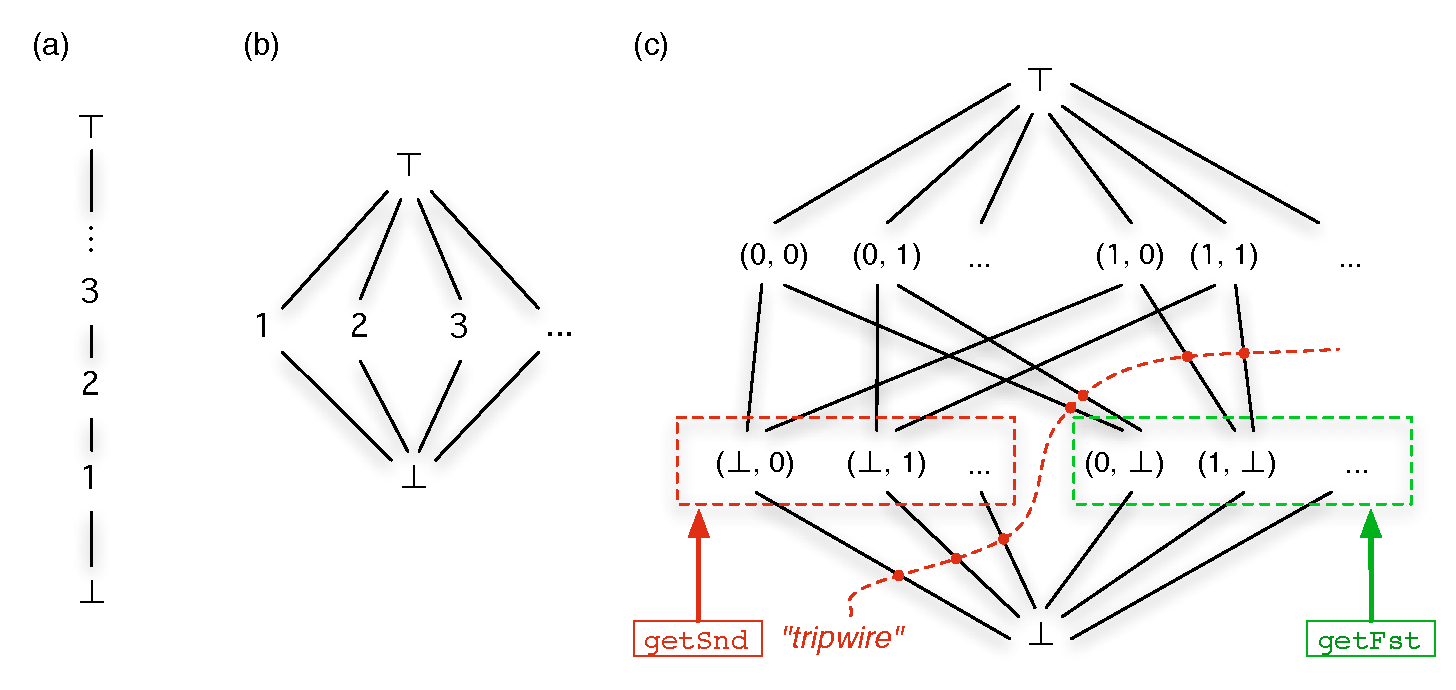
\includegraphics[width=0.75\textwidth]{figures/example-lvar-lattices.pdf} 
  \caption{Example LVar lattices: (a) positive integers ordered by
    $\leq$; (b) IVar containing a positive integer; (c) pair of
    natural-number-valued IVars, annotated with example threshold sets
    that would correspond to a blocking read of the first or second
    element of the pair.  Any state transition crossing the
    ``tripwire'' for \lstinline{getSnd} causes it to unblock and
    return a result.}

  \label{f:lattice-examples}
\end{figure}

Figure~\ref{f:lattice-examples} gives three examples of lattices for
common data structures.  The simplest example of a useful lattice is
one that represents the state space of a single-assignment variable
(an IVar).  A natural-number-valued IVar, for instance, would
correspond to the lattice in Figure~\ref{f:lattice-examples}(b), that
is, $(\lbrace \top, \bot \rbrace \cup \mathbb{N}, \userleq, \bot,
\top)$, where $\userleq$ is defined by setting $\bot \userleq d
\userleq \top$ and $d \userleq d$ for all $d \in D$.  This is a
lattice of height three and infinite width, where the naturals are
arranged horizontally.  After the initial write of some $n \in
\mathbb{N}$, any further conflicting writes would push the state of
the IVar to $\top$ (an error).  For instance, if one thread writes $2$
and another writes $1$ to an IVar (in arbitrary order), the second of
the two writes would result in an error because $2 \sqcup 1 = \top$.

In the lattice of Figure~\ref{f:lattice-examples}(a), on the other
hand, the $\top$ element can never be reached, because the least upper
bound of any two writes is just the maximum of the two.  For instance,
if one thread writes $2$ and another writes $1$, the resulting state
will be $2$, since $2 \sqcup 1 = 2$.  Here, the unreachability of
$\top$ models the fact that no conflicting updates can occur to the
LVar.

\subsection{Freezing}
 
To model freezing, the representation of an LVar must include
information about whether it is ``frozen'' or not.  Thus, in our model
an LVar's \emph{state} is a pair $\state{d}{\status}$, where $d$ is an
element of the application-specific set $D$ and $\status$ is a
``status bit'' of either $\frozentrue$ or $\frozenfalse$.  We can
define an ordering $\leqp$ on LVar states $\state{d}{\status}$ in
terms of the application-specific ordering $\userleq$ on elements of
$D$.  Every element of $D$ except $\top$ corresponds to a value at
which the LVar is ``freezable''.  Informally:
\begin{itemize}
\item Two unfrozen states are ordered according to the
  application-specific $\userleq$; that is, $\state{d}{\frozenfalse}
  \leqp \state{d'}{\frozenfalse}$ exactly when $d \userleq d'$.
\item Two frozen states do not have an order, unless they are equal:
  $\state{d}{\frozentrue} \leqp \state{d'}{\frozentrue}$ exactly when
  $d = d'$.
\item An unfrozen state $\state{d}{\frozenfalse}$ is less than or
  equal to a frozen state $\state{d'}{\frozentrue}$ exactly when $d
  \userleq d'$.
\item The only situation in which a frozen state is less than an
  unfrozen state is if the unfrozen state is $\top$; that is,
  $\state{d}{\frozentrue} \leqp \state{d'}{\frozenfalse}$ exactly when
  $d' = \top$.
\end{itemize}
The addition of status bits to the application-specific lattice
results in a new lattice $(D_p, \leqp, \botp, \topp)$, and we write
$\lubp{}{}$ for the least upper bound operation that $\leqp$ induces.

\subsection{Stores}

During the evaluation of $\lambdaLVish$ programs, a \emph{store} $S$
keeps track of the states of LVars.  Each LVar is represented by a
binding from a location $l$, drawn from a set $\Loc$, to its state,
which is some pair $\state{d}{\status}$ from the set $D_p$.

We use the notation $\extS{S}{l}{d}{\status}$ to denote extending $S$
with a binding from $l$ to $\state{d}{\status}$.  If $l \in \dom{S}$,
then $\extS{S}{l}{d}{\status}$ denotes an update to the existing
binding for $l$, rather than an extension.  We can also denote a store
by explicitly writing out all its bindings, using the notation
$\store{\storebinding{l_1}{d_1}{\status_1},
  \storebinding{l_2}{d_2}{\status_2}, \dots}$.  It is straightforward
to lift the $\leqp$ operations defined on elements of $D_p$ to a
$\leqstore{}{}$ operation defined on stores.  Stores ordered by
$\leqstore{}{}$ also form a lattice (with bottom element $\emptyset$
and top element $\topS$); we write $\lubstore{}{}$ for the induced lub
operation. If, for example,
\[ \lubp{\state{d_1}{\status_1}}{\state{d_2}{\status_2}} = \topp, \]
then
\[ \lubstore{\store{\storebinding{l}{d_1}{\status_1}}}{\store{\storebinding{l}{d_2}{\status_2}}} =
\topS. \] A store containing a binding
$\storebinding{l}{\top}{\status}$ can never arise during the execution
of an $\lambdaLVish$ program, because, as we will see in
Section~\ref{subsection:newputget}, an attempted @put@ that would
take the value of $l$ to $\top$ will raise an error.

\FigLambdaLVishGrammar

\FigLambdaLVishSemantics

\newpage

\subsection{The $\lambdaLVish$ language}

The syntax and operational semantics of the $\lambdaLVish$ calculus
appear in Figures \ref{f:lambdaLVish-syntax} and
\ref{f:lambdaLVish-semantics}, respectively.  As we have noted, both
the syntax and semantics are parameterized by the lattice $(D,
\userleq, \bot, \top)$.  The reduction relation $\parstepsto$ is
defined on \emph{configurations} $\config{S}{e}$ comprising a store
and an expression.  The \emph{error configuration}, written $\error$,
is a unique element added to the set of configurations, but we
consider $\config{\topS}{e}$ to be equal to $\error$ for all
expressions $e$.  The metavariable $\conf$ ranges over configurations.

$\lambdaLVish$ uses a reduction semantics based on evaluation
contexts.  The {\sc E-Eval-Ctxt} rule is a standard context rule,
allowing reductions to apply within a context.  The choice of context
determines where evaluation can occur; in $\lambdaLVish$, the order of
evaluation is nondeterministic (that is, a given expression can
generally reduce in more than one way), and so it is generally
\emph{not} the case that an expression has a unique decomposition into
redex and context.  For example, in an application $\app{e_1}{e_2}$,
either $e_1$ or $e_2$ might reduce first.  The nondeterminism in
choice of evaluation context reflects the nondeterminism of scheduling
between concurrent threads, and in $\lambdaLVish$, the arguments to
@get@, @put@, @freeze@, and application expressions are
\emph{implicitly} evaluated concurrently.

Arguments must be fully evaluated, however, before function
application ($\beta$-reduction, modeled by the {\sc E-Beta} rule) can
occur.  We can leverage this property to define $\LETPAR$ as syntactic
sugar:
\[
\LETPAR ~x = e_1;~~y = e_2~\IN~e_3 \;\;\defeq\;\;
\app{(\app{(\lam{x}{(\lam{y}{e_3})})}{e_1})}{e_2}
\]
Because we do not reduce under $\lambda$-terms, we can sequentially
compose $e_1$ before $e_2$ by writing $\letexp{\_}{e_1}{e_2}$, which
desugars to $\app{(\lam{\_}{e_2})}{e_1}$.  Sequential composition is
useful, for instance, when allocating a new LVar before beginning a
set of side-effecting @put@/@get@/@freeze@ operations on it.

\subsection{Semantics of $\NEW$, $\PUT$, and $\GET$}\label{subsection:newputget}

In $\lambdaLVish$, the @new@, @put@, and @get@ operations respectively
create, write to, and read from LVars in the store:
\begin{itemize}
\item @new@ (implemented by the {\sc E-New} rule) extends the store
  with a binding for a new LVar whose initial state is $(\bot,
  \frozenfalse)$, and returns the location $l$ of that LVar (\ie, a
  pointer to the LVar).
\item @put@ (implemented by the {\sc E-Put} and {\sc E-Put-Err} rules)
  takes a pointer to an LVar and a new lattice element $d_2$ and
  updates the LVar's state to the {\em least upper bound} of the
  current state and $\state{d_2}{\frozenfalse}$, potentially pushing
  the state of the LVar upward in the lattice.  Any update that would
  take the state of an LVar to $\topp$ results in the program
  immediately stepping to $\error$.
\item @get@ (implemented by the {\sc E-Get} rule) performs a blocking
  threshold read.  It takes a pointer to an LVar and a \emph{threshold
    set} $P$, which is a non-empty set of LVar states that must be
  \emph{pairwise incompatible}, expressed by the premise $\incomp{P}$.
  A threshold set $P$ is pairwise incompatible iff the lub of any two
  distinct elements in $P$ is $\topp$.  If the LVar's state $p_1$ in
  the lattice is {\em at or above} some $p_2 \in P$, the @get@
  operation unblocks and returns $p_2$.  Note that $p_2$ is a unique
  element of $P$, for if there is another $p'_2 \neq p_2$ in the
  threshold set such that $p'_2 \leqp p_1$, it would follow that
  $\lubp{p_2}{p'_2} = p_1 \neq \topp$, which contradicts the
  requirement that $P$ be pairwise incompatible.\footnote{Although
    $\incomp{P}$ is given as a premise of the {\sc E-Get} reduction
    rule (suggesting that it is checked at runtime), in the LVish
    library implementation threshold sets are not written explicitly,
    and it is the data structure author's responsibility to ensure
    that any provided read operations have threshold semantics.}
\end{itemize}
Is the @get@ operation deterministic?  Consider two lattice elements
$p_1$ and $p_2$ that have no ordering and have $\topp$ as their lub,
and suppose that @put@s of $p_1$ and $p_2$ and a @get@ with
$\setof{p_1, p_2}$ as its threshold set all race for access to an LVar
$lv$.  Eventually, the program is guaranteed to raise an exception,
because $\lubp{p_1}{p_2} = \topp$, but in the meantime,
$\getexp{lv}{\setof{p_1, p_2}}$ could return either $p_1$ or $p_2$.
Therefore, @get@ \emph{can} behave nondeterministically---but this
behavior is not observable in the final answer of the program, which
is guaranteed to subsequently raise an exception.

As an example of a threshold read, consider an LVar $\mathit{lv}$
whose states form a lattice of \emph{pairs} of natural-number-valued
IVars; that is, $\mathit{lv}$ is a pair $(m, n)$, where $m$ and $n$
both start as $\bot$ and may each be updated once with a non-$\bot$
value, which must be some natural number.  This lattice is shown in
Figure~\ref{f:lattice-examples}(c).  We can then define $\GETFST$ and
$\GETSND$ operations for reading from the first and second entries of
$\mathit{lv}$:
\begin{align*}
\getfstexp{p} & \defeq \getexp{p}{\stateset{(m, \bot) \setsep m \in
    \mathbb{N}}} \\
\getsndexp{p} & \defeq \getexp{p}{\stateset{(\bot, n) \setsep n \in
    \mathbb{N}}}
\end{align*}
This allows us to write programs like the following:
\begin{equation*}
\begin{split}
& \LETPAR ~\_ = \putexp{\mathit{lv}}{(\bot, 4)} \\
&  \letparspace ~\_ = \putexp{\mathit{lv}}{(3, \bot)} \\
&  \letparspace ~x = \getsndexp{\mathit{lv}} \\
&  \letspace \IN~x
\end{split}
\label{e:lvar-example-4}
\end{equation*}
In the call $\getsndexp{\mathit{lv}}$, the threshold set is
$\setof{(\bot, 0), (\bot, 1), \dots}$, an infinite set.  There is no
risk of nondeterminism because the elements of the threshold set are
\emph{pairwise incompatible} with respect to $\mathit{lv}$'s lattice:
informally, since the second entry of $\mathit{lv}$ can only be
written once, no more than one state from the set $\setof{(\bot, 0),
  (\bot, 1), \dots}$ can ever be reached.  The call,
$\getsndexp{\mathit{lv}}$ may unblock and return $(\bot, 4)$ any time
after the second entry of $\mathit{lv}$ has been written, regardless
of whether the first entry has been written yet.  It is therefore
possible to use LVars to safely read parts of an incomplete data
structure---say, an object that is in the process of being initialized
by a constructor.

\subsection{Semantics of freezing and event handling}

The $\lambdaLVish$ calculus includes a simple form of @freeze@ that
immediately freezes an LVar (see {\sc E-Freeze-Simple}).  More
interesting is the $\FAW$ primitive, which models the use of freezing
together with event handling.  The expression $\freezeafter{e_{\rm
    lv}}{e_{\rm events}}{e_{\rm cb}}$ has the following semantics:
\begin{itemize}
\item It attaches the callback $e_{\rm cb}$ to the LVar $e_{\rm lv}$.
  The expression $e_{\rm events}$ must evaluate to a event set $Q$;
  the callback will be executed, once, for each lattice element in $Q$
  that the LVar's state reaches or surpasses.  The callback $e_{\rm
    cb}$ is a function that takes a lattice element as its argument.
  Its return value is ignored, so it runs solely for effect.  For
  instance, a callback might itself do a @put@ to the LVar to which it
  is attached, triggering yet more callbacks.
\item If the handler reaches a quiescent state, the LVar $e_{\rm lv}$
  is frozen, and its \emph{exact} state is returned (rather than an
  underapproximation of the state, as with @get@).
\end{itemize}
\noindent
To keep track of the running callbacks, $\lambdaLVish$ uses an
auxiliary form,
\[
   \freezeafterfull{l}{Q}{\lam{x}{e_0}}{\setof{e, \dots}}{H}
\]
where:
\begin{itemize}
\item The value $l$ is the LVar being handled/frozen;
\item The set $Q$ (a subset of the lattice $D$) is the event set;
\item The value $\lam{x}{e_0}$ is the callback function;
\item The set of expressions $\setof{e, \dots}$ are the running
  callbacks; and
\item The set $H$ (a subset of the lattice $D$) represents those
  values in $Q$ for which callbacks have already been launched.
\end{itemize}
Due to the use of evaluation contexts, any running callback can
execute at any time, as if each is running in its own thread.  The
rule {\sc E-Spawn-Handler} launches a new callback thread any time the
LVar's current value is at or above some element in $Q$ that has not
already been handled.  This step can be taken nondeterministically at
any time after the relevant @put@ has been performed.

The rule {\sc E-Freeze-Final} detects quiescence by checking that two
properties hold.  First, every event of interest (lattice element in
$Q$) that has occurred (is bounded by the current LVar state) must be
handled (be in $H$).  Second, all existing callback threads must have
terminated with a value.  In other words, every enabled callback has
completed.  When such a quiescent state is detected, {\sc
  E-Freeze-Final} freezes the LVar's state.  Like {\sc
  E-Spawn-Handler}, the rule can fire at any time,
nondeterministically, that the handler appears quiescent---a transient
property!  But after the LVar is frozen, any further @put@s that would
have enabled additional callbacks will instead raise $\error$ by way
of the {\sc E-Put-Err} rule.

Therefore, freezing is a way of ``betting'' that once a collection of
callbacks have completed, no further @put@s that change the LVar's
value will occur.  For a given run of a program, either all @put@s to
an LVar arrive before it has been frozen, in which case the value
returned by $\FAW$ is the lub of those values, or some @put@ arrives
after the LVar has been frozen, in which case the program will step
to $\error$.  And thus we have arrived at \emph{quasi-determinism}: a
program will always either evaluate to the same answer or it will
raise an exception.

To ensure that we will win our bet, we need to guarantee that
quiescence is a \emph{permanent} state, rather than a transient
one---that is, we need to perform all @put@s either prior to $\FAW$,
or by the callback function within it (as will be the case for
fixpoint computations).  In practice, freezing is usually the last
step of an algorithm, permitting its result to be extracted. Our
implementation provides a special \termfont{runParThenFreeze} function
that does so, and thereby guarantees full determinism.

\subsection{Quasi-determinism proof outline}

The proof of quasi-determinism for $\lambdaLVish$ formalizes the claim
in Section~\ref{s:intro} that, for a given program, although some
executions may raise exceptions, all executions that produce a final
result will produce the same final result.  In this section, I give
the statements of the main quasi-determinism theorem and the two most
important supporting lemmas.  The statements of the remaining lemmas,
and proofs of all our theorems and lemmas, are included in our
technical report \cite{Freeze-TR}.

The main result, Theorem~\ref{thm:quasi-determinism}, says that if two
executions starting from a configuration $\conf$ terminate in
configurations $\conf'$ and $\conf''$, then $\conf'$ and $\conf''$ are
the same configuration, or one of them is $\error$.

\ThmQuasiDeterminism

\noindent Theorem~\ref{thm:quasi-determinism} follows from a series of
\emph{quasi-confluence} lemmas.  The most important of these, Strong
Local Quasi-Confluence
(Lemma~\ref{lem:strong-local-quasi-confluence}), says that if a
configuration steps to two different configurations, then either there
exists a single third configuration to which they both step (in at
most one step), or one of them steps to $\error$.  Additional lemmas
generalize Lemma~\ref{lem:strong-local-quasi-confluence}'s result to
multiple steps by induction on the number of steps, eventually
building up to Theorem~\ref{thm:quasi-determinism}.

\LemStrongLocalQuasiConfluence

\noindent In order to show
Lemma~\ref{lem:strong-local-quasi-confluence}, we need a ``frame
property'' for $\lambdaLVish$ that captures the idea that independent
effects commute with each other.  Lemma~\ref{lem:independence}, the
Independence lemma, establishes this property.  Consider an expression
$e$ that runs starting in store $S$ and steps to $e'$, updating the
store to $S'$.  The Independence lemma allows us to make a
double-edged guarantee about what will happen if we run $e$ starting
from a larger store $\lubstore{S}{S''}$: first, it will update the
store to $\lubstore{S'}{S''}$; second, it will step to $e'$ as it did
before.  Here $\lubstore{S}{S''}$ is the least upper bound of the
original $S$ and some other store $S''$ that is ``framed on'' to $S$;
intuitively, $S''$ is the store resulting from some other
independently-running computation.

\LemIndependence

\noindent Lemma~\ref{lem:independence} requires as a precondition that
the stores $\lubstore{S'}{S''}$ and $S$ are \emph{equal in
  status}---that, for all the locations shared between them, the
status bits of those locations agree.  This assumption rules out
interference from freezing.  Finally, the store $S''$ must be
\emph{non-conflicting} with the original transition from
$\config{S}{e}$ to $\config{S'}{e'}$, meaning that locations in $S''$
cannot share names with locations newly allocated during the
transition; this rules out location name conflicts caused by
allocation.

\DefEqualStatus

\DefNonConflicting

\section{Joining forces: LVars and conflict-free replicated data types}\label{s:crdts}

In this section, I discuss the relationship between the LVars model
I've described and the concept of \emph{conflict-free replicated data
  types}, and explain how I will leverage this relationship.

\subsection{Replication and eventual consistency}

Distributed systems typically involve \emph{replication} of data
objects across a number of physical locations.  Replication is of
fundamental importance in such systems: it makes the system more
robust to data loss and allows for good data locality.  Given the
importance and ubiquity of replication, it would be convenient if
systems of distributed, replicated objects behaved indistinguishably
from the more familiar programming model in which all data is on one
machine and all computation takes place there.  Unfortunately, this is
not the case.  The well-known \emph{CAP
  theorem}~\cite{gilbert-lynch-cap} of distributed computing describes
a three-way trade-off among
\begin{itemize}
\item consistency, in which every replica sees the same information;
\item availability, in which all information is available for both
  reading and writing by all replicas; and
\item partition tolerance, in which the system is robust to parts of
  it being unable to communicate with one another.
\end{itemize}
An (oversimplified, but useful to a first approximation)
interpretation of the CAP theorem is the slogan, ``Consistency,
availability, and partition tolerance: pick at most two.''  In
practice, real systems must be robust to network partitions and hence
must compromise on at least one of consistency or availability.
Moreover, though, consistency, availability, and partition tolerance
are not binary properties; rather than having, for instance, either
perfect availability or no availability at all, we can choose how much
availability a system must have, then allow less consistency
accordingly.  \emph{Highly available} distributed systems (\eg,
Dynamo~\cite{dynamo}) give up on strict consistency in favor of
\emph{eventual consistency}~\cite{vogels-ec}, in which replicas may
not always agree, but if updates stop arriving, all replicas will
\emph{eventually} come to agree.

\subsection{Resolving conflicts between replicas}

How can eventually consistent systems ensure that all replicas of an
object come to agree?  In particular, if replicas differ, how do we
determine which is ``right''?  As a straw man proposal, we could
vacuously satisfy the definition of eventual consistency by setting
all replicas to some pre-determined value---but then, of course, we
would lose all updates we had made to any of the replicas.

As a more practical proposal, we could try to determine which replica
was written most recently, then declare the last written replica the
winner.  But this approach is also less than ideal: even if we had a
way of perfectly synchronizing clocks between replicas and could
always determine which replica was written most recently, having the
last write win might not make sense from a \emph{semantic} point of
view.  The developers of Dynamo, Amazon's distributed key-value store,
acknowledge this in their discussion of application-specific
mechanisms for resolving conflicts between replicas~\cite{dynamo}:
\begin{quote}
  The next design choice is who performs the process of conflict
  resolution. This can be done by the data store or the
  application. If conflict resolution is done by the data store, its
  choices are rather limited. In such cases, the data store can only
  use simple policies, such as ``last write wins'', to resolve
  conflicting updates. On the other hand, since the application is
  aware of the data schema it can decide on the conflict resolution
  method that is best suited for its client’s experience. For
  instance, the application that maintains customer shopping carts can
  choose to ``merge'' the conflicting versions and return a single
  unified shopping cart.
\end{quote}
In other words, we can take advantage of the fact that, for a
particular application, we know something about the meaning of the
data we are storing, and then parameterize the data store by a
pluggable, application-specific conflict resolution operation.

This notion of application-specific conflict resolution is not without
its problems, especially if implemented in an ad-hoc
way.\footnote{Indeed, as noted in the Dynamo article~\cite{dynamo},
  Amazon's shopping cart presents an anomaly whereby an item removed
  from a cart may re-appear!}  Fortunately, we need not implement it
in an ad-hoc way: \emph{conflict-free replicated data types}
(CRDTs)~\cite{crdts, crdts-tr} give us a simple mathematical framework
for reasoning about and enforcing the eventual consistency of
replicated objects in a distributed system.  In the following
sections, I review the basics of CRDTs from the work of Shapiro
\etal~\cite{crdts, crdts-tr}, then discuss the relationship between
CRDTs and LVars.

\subsection{Eventual consistency and CRDTs}

Before discussing CRDTs, we must formally define eventual consistency.
Shapiro \etal~define an \emph{eventually consistent} object as one
that has the property of \emph{convergence}: all correct replicas of
the object to which the same updates have been delivered eventually
have equivalent state.  Along with convergence, they give two other
conditions that are required for eventual consistency: \emph{eventual
  delivery}, meaning that all replicas receive all update messages,
and \emph{termination}, meaning that all method executions terminate
(see below for more on methods).

Shapiro \etal~further define a \emph{strongly eventually consistent}
(SEC) object as one that is eventually consistent and, in addition to
being merely convergent, is \emph{strongly convergent}, meaning that
correct replicas to which the same updates have been delivered have
equivalent state.\footnote{Contrast with ordinary convergence, in
  which replicas only \emph{eventually} have equivalent state.  An
  object might be convergent but not strongly convergent if, for
  example, the system executes an update on some replica and then
  later rolls back the update after discovering that it conflicts with
  another.}  A \emph{conflict-free replicated data type} (CRDT), then,
is a data type (\ie, a specification for an object) satisfying certain
conditions that are sufficient to guarantee that the object is SEC.
(The term ``CRDT'' is used interchangeably to mean a specification for
an object, or an object meeting that specification.)

There are two ``styles'' of specifying a CRDT: \emph{state-based},
also known as \emph{convergent}\footnote{This terminology is somewhat
  unfortunate: the definitions of convergence and strong convergence
  above pertain to \emph{all} CRDTs, not just those specified in the
  ``convergent'' style!}; or \emph{operation-based} (or ``op-based''),
also known as \emph{commutative}.  CRDTs specified in the state-based
style are also called \emph{convergent replicated data types},
abbreviated \emph{CvRDTs}, while those specified in the op-based style
are also called \emph{commutative replicated data types}, abbreviated
\emph{CmRDTs}.  The state-based (CvRDT) style is closer to the LVars
model, although, as we will see, CmRDTs can emulate CvRDTs, and vice
versa.

\lk{The paper is hard to read because they don't actually define a
  CvRDT.  They define a ``monotonic semilattice object'', which, by
  definition, meets the ``monotonic semilattice property'', I guess.
  Then they show that any state-based object that satisfies the
  monotonic semilattice property is SEC, but the name of that theorem
  is ``CvRDT''.  So I guess that means that a CvRDT satisfies the
  monotonic semilattice property and is therefore SEC.  Another way to
  do this would have been to define a CvRDT as meeting the monotonic
  semilattice property and then proving that a CvRDT is SEC.}

\subsection{CvRDTs and LVars}

Shapiro \etal~specify a \emph{state-based object} as a tuple $(S, s^0,
q, u, m)$, where $S$ is a set of states, $s^0$ is the initial state,
$q$ is the \emph{query method}, $u$ is the \emph{update method}, and
$m$ is the \emph{merge method}.  Objects are replicated across some
finite number of processes, with one replica at each process.  We
assume that each replica begins in the initial state $s^0$.  The state
of a local replica may be queried via the method $q$ and updated via
the method $u$.  Methods execute locally, at a single replica, but the
merge method $m$ can merge the state from a remote replica with the
local replica; we assume that every replica
regularly\footnote{``Infinitely often'', according to Shapiro \etal}
sends its local state to some other replica, and that eventually every
update reaches every replica, whether directly or indirectly.

A \emph{state-based} or \emph{convergent} replicated data type (CvRDT)
is a state-based object equipped with a partial order $\leq$, written
$(S, \leq, s^0, q, u, m)$, that has the following properties:
\begin{itemize}
\item $S$ forms a join-semilattice ordered by $\leq$.
\item The merge method $m$ computes the least upper bound of the two
  states with respect to $\leq$.
\item State is \emph{inflationary} across updates: if $u$ updates a
  state $s$ to $s'$, then $s \leq s'$.
\end{itemize}
Shapiro \etal~show that a state-based object that meets the criteria
for a CvRDT is SEC~\cite{crdts}.  CvRDTs have much in common with
LVars, but they differ in the following ways:
\begin{itemize}
\item In the CvRDT model, there is no notion of threshold reads; the
  query operation $q$ reads the exact contents of its local replica,
  and therefore different replicas may see different states at the
  same time, if not all updates have been propagated yet.
\item In the LVars model, there is no ``update'' operation that is
  distinct from ``merge''---since LVar @put@s compute the least upper
  bound of the old and new values, an LVar update is the equivalent of
  a CvRDT merge operation.
\item In the LVars model, we do not have to contend with replication!
  The LVars model is a shared-memory model, and when an LVar is
  updated, all reading threads immediately see the update.
\end{itemize}
These differences, however, suggest some possibilities for extending
both the LVars and CvRDT models.  I propose to do the following:
\begin{itemize}
\item Extend the definition of CvRDTs to add a mechanism for
  specifying LVar-style threshold reads---say, by adding a new $g$
  (for ``get'') operation.  Threshold reads should guarantee that the
  order in which information is added to a CvRDT cannot be observed,
  ensuring a greater degree of consistency at the price of read
  availability.  My hypothesis is that, for a CvRDT where \emph{all}
  reads are threshold reads made via the $g$ operation, we can
  guarantee something more than strong convergence: all reads will be
  consistent.  I will formally define and prove this \emph{query
    consistency} property for extended CvRDTs.  In practice, though, a
  combination of threshold reads and regular reads may make the most
  sense.
\item Extend the LVars model to allow non-lub update operations---that
  is, allow update operations other than @put@---while nevertheless
  preserving determinism.  In fact, the @bump@ operation discussed in
  Section~\ref{ss:lvish}---which is already a useful part of the LVish
  library, but not yet formalized or proved deterministic in the
  setting of $\lambdaLVish$---is just such a non-lub update operation.
  I will parameterize the definition of $\lambdaLVish$ by an
  inflationary function $f$, add a @bump@ expression to the
  $\lambdaLVish$ syntax, add (something like) the following rule {\sc
    E-Bump} to the operational semantics, and prove determinism for
  the resulting extended language:
\begin{mathpar}
    \inferrule*[lab=E-Bump]
        {S(l) = \state{d_1}{\frozenfalse} \\ d_1 \userleq f(d_1) \\ f(d_1) \neq \top}
        {\config{S}{\bumpexp{l}} \parstepsto
          \config{\extSRaw{S}{l}{\state{f(d_1)}{\frozenfalse}}}{\unit}}
\end{mathpar}
  Support for inflationary non-lub updates should make the LVars model
  more expressive (while retaining determinism) and bring the LVars
  and CvRDT models closer together.
\end{itemize}
Finally, there is another interesting possibility, which I discuss
next: the existence of CRDTs that allow non-monotonic operations
suggests a way of extending LVars to allow not only non-lub updates,
but \emph{non-monotonic} updates.

\subsection{CmRDTs and non-monotonic updates}

As mentioned above, CmRDTs and CvRDTs can emulate each other.
However, unlike CvRDTs, which are state-based objects specified using
partial orders and for which replicas converge by exchanging
information about their local \emph{state}, CmRDTs are \emph{op-based}
objects, and their replicas converge by telling each other \emph{what
  operations have taken place} locally.

Shapiro \etal~specify an \emph{op-based object} as a tuple $(S, s^0,
q, t, u, P)$, where, as before, $S$, $s^0$, and $q$ are respectively
the set of states, the initial state, and the query method. $t$ and
$u$ are the \emph{prepare-update} method and the \emph{effect-update}
method, respectively: updating a local replica involves executing $t$
locally, immediately followed by $u$ locally, and so we denote an
update as a pair $(t, u)$.  However, the effect-update method $u$ also
executes at all other replicas.  The local replica delivers the
effect-update to the other replicas using a communication protocol,
specified by the \emph{delivery precondition} $P$, that makes certain
assumptions about the reliability and consistency of the underlying
network.

For present purposes, the details of $P$ are not important; the
important thing to note is that an op-based object has no merge
method, and so the above definition of CvRDTs, in which the merge
method $m$ computes a least upper bound, cannot apply to op-based
objects.  Instead, Shapiro \etal~define an \emph{op-based} or
\emph{commutative} replicated data type (CmRDT) to be an op-based
object with the property that \emph{all concurrent updates commute}.
We say that updates $(t, u)$ and $(t', u')$ commute iff, for any
reachable replica state $s$ where both $u$ and $u'$ are \emph{enabled}
by the delivery precondition $P$ (that is, $P(s, u)$ and $P(s, u')$
are both true), the following conditions hold:
\begin{itemize}
  \item $u$ remains enabled by $P$ after $u'$ has executed,
  \item $u'$ remains enabled by $P$ after $u$ has executed, and
  \item the state resulting from executing $u$ followed by $u'$
    starting from $s$ is equivalent to the state resulting from
    executing $u'$ followed by $u$ starting from $s$.
\end{itemize}
As an example of a CmRDT, Shapiro \etal~give an op-based specification
for an \emph{OR-Set} (``observed-remove set'') data structure.
OR-Sets are sets that support removal as well as addition of elements
(because concurrent adds and removes commute).

Just as a state-based object that meets the CvRDT criteria is SEC,
Shapiro \etal~show that an op-based object that meets the criteria for
a CmRDT is SEC~\cite{crdts}.  Moreover, they give a constructive proof
that CmRDTs and CvRDTs can emulate each other by showing a general way
to construct an equivalent CvRDT given a CmRDT, and vice versa.  In
the CmRDT-to-CvRDT direction of the proof, \emph{known updates}
(operations that have taken place locally) and \emph{delivered
  updates} (local operations that have been broadcast by an
effect-update) are modeled as two grow-only sets.

Since CmRDT operations do not have to update the state $s$
monotonically with respect to a lattice, it is possible to implement
CmRDTs (and therefore equivalent CvRDTs!) that allow ``non-monotonic''
operations.  (The state of the \emph{emulating} CvRDT, however,
\emph{does} grow monotonically with respect to \emph{its} partial
order; otherwise, it would not be a CvRDT.) For example, it should be
possible to use Shapiro \etal's emulation construction to emulate
their op-based OR-Set specification with an equivalent state-based
one.

Shapiro \etal~also give examples showing that, for certain data types,
it is possible to \emph{directly} specify a CvRDT that allows
non-monotonic operations.  A set that allows both additions and
removals, for instance, can be specified directly as a CvRDT; the
trick is to encode the set as \emph{two} grow-only sets, one for
elements added and one for elements removed.  This data structure is
known as a \emph{2P-Set} (for ``two-phase set'').  However, with such
an encoding, once an element is removed, it can never be added again
thereafter!  \emph{Counters}, however, do not suffer from the same
problem: we can encode a counter that allows both increments and
decrements directly as a CvRDT using two grow-only counters, one for
increments and one for decrements, and having the query method $q$
return the difference of the two.  The resulting data structure is
called a \emph{PN-Counter} (for ``positive/negative counter'').

I refer to CvRDTs that allow non-monotonic operations as
\emph{monotonic emulations} of non-monotonic data structures, whether
they use Shapiro \etal's CmRDT-to-CvRDT construction or whether they
are directly implemented as CvRDTs.  However, queries can observe the
order of updates---and allowing non-monotonic operations aggravates
this observability problem.  Next, I consider what it would take to
prevent the order of updates from being observed even in the presence
of non-monotonic updates.

\subsection{Threshold reads of non-monotonic data structures}

What would it mean to perform a threshold read on a data structure
that allows non-monotonic operations?  At first glance, threshold
reads of non-monotonic data structures would seem to pose a problem
for determinism. If only monotonic operations are allowed, as is the
case for LVars, then whether or not a given @get@ operation unblocks
is the same from run to run (although it may unblock at different
times, depending on scheduling).  But if the state of an LVar were
allowed to move both up and down in a lattice, this would no longer be
the case. For instance, if a @get@ operation were thresholded on an
element that was added to and later removed from a set, then the @get@
might block forever, or not, depending on whether it ran after or
before the element's removal.

One option for resolving this dilemma is to give up on threshold reads
entirely for data structures that allow non-monotonic operations.
However, it is also worth considering another option, which is to
change the semantics of threshold reads to reveal even less
information than they do now.  In the existing LVars model, when a
@get@ returns, it is a guarantee that the contents of the LVar it is
reading are at or above a certain point in the lattice: ``The contents
of this LVar are at least $x$.''  But for non-monotonic data
structures, we could, instead, have the following guarantee:
``\emph{There exists a schedule} under which the contents of this data
structure \emph{could have at one time} been $x$.''  Although this
latter guarantee is much weaker, there still may be situations in
which it is useful.  Changing the semantics of threshold reads in this
way would allow thresholding on the state of a CmRDT directly.

Finally, yet another possibility is to leave the semantics of
threshold reads as they are and threshold directly on the
(monotonically growing) state of a CvRDT that is the \emph{monotonic
  emulation} of a non-monotonic data structure.  Such a CvRDT might be
an emulation of a CmRDT, or it might be a non-monotonic data structure
encoded directly as a CvRDT, such as a PN-Counter.  Threshold reads of
the emulating (monotonically growing) data structure, rather than the
emulated (non-monotonic) one, could leverage what we know about the
implmementation details of the emulation to allow unusual kinds of
queries.  It might be useful, for instance, to know when a PN-Counter
has been decremented at least $n$ times, regardless of its total.  If
so, we could easily threshold on the size of the internal grow-only
decrement counter using a standard threshold read.

The last of these possibilities seems to fit well into the LVars model
because it does not require changing the monotonic semantics of LVars.
Therefore, I propose to implement LVar-based versions of 2P-Sets and
PN-Counters, using a monotonic emulation for the non-monotonic
operations, and exposing @get@ operations that correspond to standard
threshold reads, but threshold on the emulating monotonic data
structure.

\section{Related work}\label{s:related}

Work on deterministic parallel programming models is long-standing.
As discussed in Section~\ref{s:intro}, the LVars model builds on long
traditions of work on parallel programming models based on
monotonically-growing shared data structures, and it provides a
framework for generalizing and unifying these existing approaches.  In
this section I describe some more recent contributions to the
literature.

As we have seen, what deterministic parallel programming models have
in common is that they all must do something to restrict access to
mutable state shared among concurrent computations so that schedule
nondeterminism cannot be observed.  Depending on the model,
restricting access to shared mutable state might involve disallowing
sharing entirely \cite{dph}, only allowing single assignments to
shared references \cite{Tesler-1968, IStructures, CnC}, allowing
sharing only by a limited form of message passing \cite{Kahn-1974},
ensuring that concurrent accesses to shared state are disjoint
\cite{dpj-oopsla}, resolving conflicting updates after the fact
\cite{concurrent-revisions-haskell11}, or some combination of these
approaches.  These constraints can be imposed at the language or API
level, within a type system, or at runtime.

\subsection{Deterministic Parallel Java (DPJ)}

DPJ \cite{dpj-oopsla, dpj-hotpar09} is a deterministic language
consisting of a system of annotations for Java code.  A sophisticated
region-based type system ensures that a mutable region of the heap is,
essentially, passed linearly to an exclusive writer, thereby ensuring
that the state accessed by concurrent threads is disjoint.  DPJ does,
however, provide a way to unsafely assert that operations commute with
one another (using the @commuteswith@ form) to enable concurrent
mutation.

The LVars model differs from DPJ in that it allows overlapping shared
state between threads as the default.  Moreover, since LVar effects
are already commutative, we avoid the need for @commuteswith@
annotations.  Finally, it is worth noting that while in DPJ,
commutativity annotations have to appear in application-level code, in
LVish only the data-structure author needs to write trusted code. The
application programmer can run untrusted code that still enjoys a
(quasi-)determinism guarantee, because only (quasi-)deterministic
programs can be expressed as LVish @Par@ computations.

More recently, Bocchino \etal~\cite{dpj-popl} proposed a type and
effect system that allows for the incorporation of nondeterministic
sections of code in DPJ.  The goal here is different from ours: while
they aim to support \emph{intentionally} nondeterministic computations
such as those arising from optimization problems like branch-and-bound
search, the quasi-determinism in LVish arises as a result of schedule
nondeterminism.

\subsection{FlowPools}

Prokopec \etal~\cite{flowpools} recently proposed a data structure
with an API closely related to LVars extended with freezing and
handlers: a FlowPool is a bag (that is, a multiset) that allows
concurrent insertions but forbids removals, a @seal@ operation that
forbids further updates, and combinators like @foreach@ that invoke
callbacks as data arrives in the pool.  To retain determinism, the
@seal@ operation requires explicitly passing the expected bag
\emph{size} as an argument, and the program will raise an exception if
the bag goes over the expected size.

While this interface has a flavor similar to that of LVars, it lacks
the ability to detect quiescence, which is crucial for expressing
algorithms like graph traversal, and the @seal@ operation is awkward
to use when the structure of data is not known in advance.  By
contrast, the @freeze@ operation on LVars does not require such
advance knowledge, but moves the model into the realm of
quasi-determinism.  Another important difference is the fact that
LVars are \emph{data structure-generic}: both our formalism and our
library support an unlimited collection of data structures, whereas
FlowPools are specialized to bags.

\subsection{Concurrent Revisions}

The Concurrent Revisions (CR)~\cite{concurrent-revisions-haskell11}
programming model uses isolation types to distinguish regions of the
heap shared by multiple mutators.  Rather than enforcing exclusive
access in the style of DPJ, CR clones a copy of the state for each
mutator, using a deterministic ``merge function'' for resolving
conflicts in local copies at join points.

In CR, variables can be annotated as being shared between a ``joiner''
thread and a ``joinee'' thread.  Unlike the least-upper-bound writes
of LVars, CR merge functions are \emph{not} necessarily commutative;
indeed, the default CR merge function is ``joiner wins''.  Determinism
is enforced by the programming model allowing the programmer to
specify which of two writing threads should prevail, regardless of the
order in which those writes arrive, and the states that a shared
variable can take on need not form a lattice.  Still, semilattices
turn up in the metatheory of CR: in particular, Burckhardt and
Leijen~\cite{semantics-concurrent-revisions} show that, for any two
vertices in a CR revision diagram, there exists a \emph{greatest
  common ancestor} state that can be used to determine what changes
each side has made---an interesting duality with our model (in which
any two LVar states have a lub).\lk{TODO: Write to them and ask them
  if it's a join-semilattice or a meet-semilattice!}

Although versioned variables in CR could model lattice-based data
structures---if they used least upper bound as their merge function
for conflicts---the programming model nevertheless differs from the
LVars model in that effects only become visible at the end of parallel
regions, as opposed to the asynchronous communication within parallel
regions that the LVars model allows.  This semantics precludes the use
of traditional lock-free data structures for representing versioned
variables.

\subsection{Bloom and Bloom$^L$}

The Bloom language for distributed database programming guarantees
eventual consistency for distributed data collections that are updated
monotonically.  The initial formulation of Bloom~\cite{bloom-cidr} had
a notion of monotonicity based on set inclusion, analogous to the
store ordering used in the proof of determinism for the (IVar-based)
CnC system~\cite{CnC}.  More recently, Conway \etal~\cite{blooml}
generalized Bloom to a more flexible lattice-parameterized system,
Bloom$^L$, in a manner analogous to our generalization from IVars to
LVars.  Bloom$^L$ combines ideas from CRDTs with \emph{monotonic
  logic}, resulting in a lattice-parameterized, confluent language
that is a close relative of LVish.  A monotonicity analysis pass rules
out programs that would perform non-monotonic operations on
distributed data collections, whereas in the LVars model, monotonicity
is enforced by the API presented by LVars.  Another difference between
Bloom($^L$) and the LVars model is that the former does not have a
notion of quasi-determinism.\lk{TODO: make sure this is the case---I
  think there might be some sort of way to unsafely peek in Bloom, but
  it's ruled out by the CALM analysis.}  Finally, since LVish is
implemented as a Haskell library (whereas Bloom($^L$) is implemented
as a domain-specific language embedded in Ruby), we can rely on
Haskell's static type system for fine-grained effect tracking and
monadic encapsulation of LVar effects.

\section{Research plan}

Together with my collaborators, I have already completed substantial
work towards my thesis:

\begin{itemize}
  \item Formally defined a parallel calculus,
    $\lambda_{\textrm{LVar}}$, that demonstrates the basic LVars model
    (with @put@ and @get@ operations); implemented it in PLT Redex;
    and proved determinism for it~\cite{LVars-paper, LVars-TR}.

  \item Formally defined the LVish calculus (called $\lambdaLVish$ in
    this proposal), which extends $\lambda_{\textrm{LVar}}$ with
    freezing and event handlers; implemented it in PLT Redex; and
    proved quasi-determinism for it~\cite{Freeze-paper, Freeze-TR}.

  \item Implemented and released the LVish Haskell library based on
    the formal LVars model~\cite{Freeze-paper}.
\end{itemize}
To complete the thesis, I plan to do the following:
\begin{itemize}
\item Formally define the semantics of @bump@ and add it to
  $\lambdaLVish$.  Prove determinism for the subset of $\lambdaLVish$
  that includes @bump@, but does not include freezing and event
  handlers (this proof should be a straightforward refactoring of the
  existing determinism proof for
  $\lambda_{\textrm{LVar}}$\footnote{Indeed, the updated version of
    the proof will be simpler because $\lambda_{\textrm{LVar}}$ has
    simultaneous parallel reductions, requiring a large amount of
    proof bookkeeping with regard to renaming of store locations,
    whereas $\lambdaLVish$ models parallelism with interleaving (as is
    the standard approach) and therefore is easier to reason about.}).
  Update the existing quasi-determinism proof for $\lambdaLVish$ to
  account for @bump@.  (Time estimate: 1 month.)

\item Extend the definition of CvRDTs to include threshold reads.
  Define and prove a query consistency property for CvRDTs extended
  thusly. (Time estimate: 2 months.)

\item Implement PN-Counters and 2P-Sets in the LVish library and
  release a new version of LVish with these extensions.  Implement at
  least one application that makes use of these CRDT-inspired
  LVars. (Time estimate: 3 months.)

\item Expand Kuper \etal~\cite{Freeze-paper} to an extended version
  for journal submission, including the above material on @bump@,
  write a new paper on my work integrating CRDTs and LVars, and
  integrate the material from these papers into the dissertation
  itself. (Time estimate: 3 months.)

\end{itemize}
This plan puts me on track to defend in September 2014.

\newpage

\bibliographystyle{plain}
\newcommand{\myname}[0]{Lindsey Kuper}
\bibliography{../latex_common/refs,../latex_common/lkuper}

\end{document}
